% -*- Mode:TeX -*-

%% IMPORTANT: The official thesis specifications are available at:
%%            http://libraries.mit.edu/archives/thesis-specs/
%%
%%            Please verify your thesis' formatting and copyright
%%            assignment before submission.  If you notice any
%%            discrepancies between these templates and the 
%%            MIT Libraries' specs, please let us know
%%            by e-mailing thesis@mit.edu

%% The documentclass options along with the pagestyle can be used to generate
%% a technical report, a draft copy, or a regular thesis.  You may need to
%% re-specify the pagestyle after you \include  cover.tex.  For more
%% information, see the first few lines of mitthesis.cls. 

%\documentclass[12pt,vi,twoside]{mitthesis}
%%
%%  If you want your thesis copyright to you instead of MIT, use the
%%  ``vi'' option, as above.
%%
%\documentclass[12pt,twoside,leftblank]{mitthesis}
%%
%% If you want blank pages before new chapters to be labelled ``This
%% Page Intentionally Left Blank'', use the ``leftblank'' option, as
%% above. 

\documentclass[12pt,twoside]{mitthesis}
\usepackage{lgrind}
%% These have been added at the request of the MIT Libraries, because
%% some PDF conversions mess up the ligatures.  -LB, 1/22/2014
\usepackage{cmap}
\usepackage[T1]{fontenc}
\pagestyle{plain}
\usepackage{graphicx}
\usepackage[hidelinks]{hyperref}
\usepackage{amsmath,mleftright}
\usepackage{amsthm}
\usepackage{amssymb}
\usepackage{enumerate}
\usepackage{multirow}

\usepackage[top=3.5cm,right=3cm,bottom=4cm,left=3cm]{geometry}
\usepackage{abstract}
\renewcommand{\absnamepos}{empty}
\usepackage[english]{babel}
\usepackage{tikz}
\usepackage{pgfplots}
\usepackage{subfig}
\usepackage{multirow}
\usepackage{pdfpages}

\usepackage{mathrsfs}
\usepackage{algorithmicx}
\usepackage{algpseudocode}
\usepackage{algorithm}
\graphicspath{
	{images/}
}
\usepackage{afterpage}

\newcommand\blankpage{%
	\null
	\thispagestyle{empty}%
	\addtocounter{page}{-1}%
	\newpage}
\newtheorem{theorem}{Theorem}
%% This bit allows you to either specify only the files which you wish to
%% process, or `all' to process all files which you \include.
%% Krishna Sethuraman (1990).

\DeclareMathOperator{\eff}{eff}
\DeclareMathOperator{\dx}{dx}
\def\startpage{
	\newpage
	\vspace*{3cm}
	\begin{center}
		
\includegraphics[width=12cm]{besm}
	\end{center}
}

\makeatletter         
\def\@maketitle{
	\raggedright
	\begin{center}
		{
\includegraphics[width = 10cm]{logopolito.jpg}}\\[8ex]
		{\Huge \bfseries \sffamily \@title }\\[4ex] 
		{\Large  \@author}\\[4ex] 
		\@date\\
\end{center}}
\makeatother


\let\cleardoublepage\clearpage

\newcommand\aeeq{\mathrel{\stackrel{\makebox[0pt]{\mbox{\normalfont\tiny a.e}}}{=}}}

\newcommand{\norm}[1]{\left\lVert#1\right\rVert}
\newcommand{\abs}[1]{\vert#1\vert}
\newcommand{\esssup}[2]{\mathop{\mathrm{ess~sup}}\limits_{#1}#2}
\newcommand{\essinf}[2]{\mathop{\mathrm{ess~inf}}\limits_{#1}#2}
\newcommand{\innerProduct}[2]{\mathop{\langle #1, #2 \rangle}}


\theoremstyle{plain}
\newtheorem{thm}{Theorem}[chapter] % reset theorem numbering for each chapter

\theoremstyle{definition}
\newtheorem{defn}[thm]{Definition} % definition numbers are dependent on theorem numbers
\newtheorem{exmp}[thm]{Example} % same for example numbers

\newtheorem{lemma}[theorem]{Lemma}
\newtheorem{corollary}[theorem]{Corollary}
\newtheorem{remark}[theorem]{Remark}
\newtheorem{notation}[theorem]{Notation}
\newtheorem{assumption}[theorem]{Assumption}


\mleftright
\begin{document}

% -*-latex-*-
% 
% For questions, comments, concerns or complaints:
% thesis@mit.edu
% 
%
% $Log: cover.tex,v $
% Revision 1.8  2008/05/13 15:02:15  jdreed
% Degree month is June, not May.  Added note about prevdegrees.
% Arthur Smith's title updated
%
% Revision 1.7  2001/02/08 18:53:16  boojum
% changed some \newpages to \cleardoublepages
%
% Revision 1.6  1999/10/21 14:49:31  boojum
% changed comment referring to documentstyle
%
% Revision 1.5  1999/10/21 14:39:04  boojum
% *** empty log message ***
%
% Revision 1.4  1997/04/18  17:54:10  othomas
% added page numbers on abstract and cover, and made 1 abstract
% page the default rather than 2.  (anne hunter tells me this
% is the new institute standard.)
%
% Revision 1.4  1997/04/18  17:54:10  othomas
% added page numbers on abstract and cover, and made 1 abstract
% page the default rather than 2.  (anne hunter tells me this
% is the new institute standard.)
%
% Revision 1.3  93/05/17  17:06:29  starflt
% Added acknowledgements section (suggested by tompalka)
% 
% Revision 1.2  92/04/22  13:13:13  epeisach
% Fixes for 1991 course 6 requirements
% Phrase "and to grant others the right to do so" has been added to 
% permission clause
% Second copy of abstract is not counted as separate pages so numbering works
% out
% 
% Revision 1.1  92/04/22  13:08:20  epeisach

% NOTE:
% These templates make an effort to conform to the MIT Thesis specifications,
% however the specifications can change.  We recommend that you verify the
% layout of your title page with your thesis advisor and/or the MIT 
% Libraries before printing your final copy.

\title{Solving Partial Differential Equations with Uncertainties Using Neural-Networks}

\author{Sajed Zarrinpour Nashroudkoli}
% If you wish to list your previous degrees on the cover page, use the 
% previous degrees command:
%       \prevdegrees{A.A., Harvard University (1985)}
% You can use the \\ command to list multiple previous degrees
%       \prevdegrees{B.S., University of California (1978) \\
%                    S.M., Massachusetts Institute of Technology (1981)}
%\department{Department of Electrical Engineering and Computer Science}

% If the thesis is for two degrees simultaneously, list them both
% separated by \and like this:
% \degree{Doctor of Philosophy \and Master of Science}
\degree{Applied Mathematics - Numerical Analysis \\ Master's}
\department{Department of Mathematics}
% As of the 2007-08 academic year, valid degree months are September, 
% February, or June.  The default is June. Changed to today date
\latinthesisdate{September 2020}
%\degreemonth{June}
%\degreeyear{1990}
%\thesisdate{May 18, 1990}

%% By default, the thesis will be copyrighted to MIT.  If you need to copyright
%% the thesis to yourself, just specify the `vi' documentclass option.  If for
%% some reason you want to exactly specify the copyright notice text, you can
%% use the \copyrightnoticetext command.  
%\copyrightnoticetext{\copyright IBM, 1990.  Do not open till Xmas.}

% If there is more than one supervisor, use the \supervisor command
% once for each.

\supervisor{Khadije Nedaiasl\\[1cm]{Advisor:\hspace*{1.5cm} Parvin Razzaghi}}{}
%\supervisor{Khadije Nedaiasl}{}

% This is the department committee chairman, not the thesis committee
% chairman.  You should replace this with your Department's Committee
% Chairman.
%\chairman{Parvin Razzaghi}{}{Chairman, Department Committee on Graduate Theses}

% Make the titlepage based on the above information.  If you need
% something special and can't use the standard form, you can specify
% the exact text of the titlepage yourself.  Put it in a titlepage
% environment and leave blank lines where you want vertical space.
% The spaces will be adjusted to fill the entire page.  The dotted
% lines for the signatures are made with the \signature command.
\maketitle
\pagenumbering{roman}
\setcounter{page}{1}
%\startpage
\blankpage
\newpage
% The abstractpage environment sets up everything on the page except
% the text itself.  The title and other header material are put at the
% top of the page, and the supervisors are listed at the bottom.  A
% new page is begun both before and after.  Of course, an abstract may
% be more than one page itself.  If you need more control over the
% format of the page, you can use the abstract environment, which puts
% the word "Abstract" at the beginning and single spaces its text.

%% You can either \input (*not* \include) your abstract file, or you can put
%% the text of the abstract directly between the \begin{abstractpage} and
%% \end{abstractpage} commands.

% First copy: start a new page, and save the page number.
%\cleardoublepage
% Uncomment the next line if you do NOT want a page number on your
% abstract and acknowledgments pages.Parvin
%\pagestyle{empty}
\section*{\centering Acknowledgments}
Foremost, I would like to thank my supervisor Dr. Khadije Nedaiasl for her continuous support during my research. She did a great deal encouraging me and helping me researching and writing this thesis.

Besides my supervisor, I would like to thank Dr. Parvin Razaghi and Dr. DehBozorgi without whom, this thesis may never have been concluded.
Also, I have special thanks to my friends, especially Maryam, who supported me in any possible way and I'm sure without them I would never come to this point. 
%Also thanks to everyone in the networks lab, it was a great sharing laboratory with all of %you during the last three years.

Last but not least, I would like to thank my family who helped me both financially and spiritually along the way.

%A part of this work had been done during the COVID-19 pandemic, when I had to live with my brother Sobhan and his wife Zohre.  

Everyone, Thanks for all your encouragements. 
\newpage
%\setcounter{savepage}{\thepage}
\begin{latinabstract}
\addcontentsline{toc}{section}{Abstract}
% $Log: abstract.tex,v $
% Revision 1.1  93/05/14  14:56:25  starflt
% Initial revision
% 
% Revision 1.1  90/05/04  10:41:01  lwvanels
% Initial revision
% 
%
%% The text of your abstract and nothing else (other than comments) goes here.
%% It will be single-spaced and the rest of the text that is supposed to go on
%% the abstract page will be generated by the abstractpage environment.  This
%% file should be \input (not \include 'd) from cover.tex.
Towards modeling the real-world phenomenons with partial differential equations that involve uncertainties, one of the major difficulties is a set of phenomena known as the curse of dimensionality. Luckily, very often the variability of physical quantities derived from the model can be captured by a few features on the coefficient fields, with what so called model reduction techniques. On the other hand, neural networks are good at finding hidden maps on the data. For example, one can use neural-networks based methods to parametrize the physical quantity of interest as a function of input coefficients. In that case, the representability of such quantity can be justified by viewing the neural networks as performing time evolution to find the solution to the model. Indeed, in this thesis, we review a surrogate forward neural network model used to solve two notable partial differential equations in engineering and physics. Also, we explain possibilities that neural networks comes forward throw looking at the mathematical analysis of a well known method, namely finite element method.
\keywords{Partial Differential Equations, Finite Difference Method, Finite Element Method, Uncertainty Quantification}


\end{latinabstract}
% Additional copy: start a new page, and reset the page number.  This way,
% the second copy of the abstract is not counted as separate pages.
% Uncomment the next 6 lines if you need two copies of the abstract
% page.
% \setcounter{page}{\thesavepage}
% \begin{abstractpage}
% % $Log: abstract.tex,v $
% Revision 1.1  93/05/14  14:56:25  starflt
% Initial revision
% 
% Revision 1.1  90/05/04  10:41:01  lwvanels
% Initial revision
% 
%
%% The text of your abstract and nothing else (other than comments) goes here.
%% It will be single-spaced and the rest of the text that is supposed to go on
%% the abstract page will be generated by the abstractpage environment.  This
%% file should be \input (not \include 'd) from cover.tex.
Towards modeling the real-world phenomenons with partial differential equations that involve uncertainties, one of the major difficulties is a set of phenomena known as the curse of dimensionality. Luckily, very often the variability of physical quantities derived from the model can be captured by a few features on the coefficient fields, with what so called model reduction techniques. On the other hand, neural networks are good at finding hidden maps on the data. For example, one can use neural-networks based methods to parametrize the physical quantity of interest as a function of input coefficients. In that case, the representability of such quantity can be justified by viewing the neural networks as performing time evolution to find the solution to the model. Indeed, in this thesis, we review a surrogate forward neural network model used to solve two notable partial differential equations in engineering and physics. Also, we explain possibilities that neural networks comes forward throw looking at the mathematical analysis of a well known method, namely finite element method.
\keywords{Partial Differential Equations, Finite Difference Method, Finite Element Method, Uncertainty Quantification}


% \end{abstractpage}
%%%%%%%%%%%%%%%%%%%%%%%%%%%%%%%%%%%%%%%%%%%%%%%%%%%%%%%%%%%%%%%%%%%%%%
% -*-latex-*-

% Some departments (e.g. 5) require an additional signature page.  See
% signature.tex for more information and uncomment the following line if
% applicable.
%% -*- Mode:TeX -*-
%
% Some departments (e.g. Chemistry) require an additional cover page
% with signatures of the thesis committee.  Please check with your
% thesis advisor or other appropriate person to determine if such a 
% page is required for your thesis.  
%
% If you choose not to use the "titlepage" environment, a \newpage
% commands, and several \vspace{\fill} commands may be necessary to
% achieve the required spacing.  The \signature command is defined in
% the "mitthesis" class
%
% The following sample appears courtesy of Ben Kaduk <kaduk@mit.edu> and
% was used in his June 2012 doctoral thesis in Chemistry. 

\begin{titlepage}
\begin{large}
This doctoral thesis has been examined by a Committee of the Department
of Chemistry as follows:

\signature{Professor Jianshu Cao}{Chairman, Thesis Committee \\
   Professor of Chemistry}

\signature{Professor Troy Van Voorhis}{Thesis Supervisor \\
   Associate Professor of Chemistry}

\signature{Professor Robert W. Field}{Member, Thesis Committee \\
   Haslam and Dewey Professor of Chemistry}
\end{large}
\end{titlepage}


%\pagestyle{plain}
  % -*- Mode:TeX -*-
%% This file simply contains the commands that actually generate the table of
%% contents and lists of figures and tables.  You can omit any or all of
%% these files by simply taking out the appropriate command.  For more
%% information on these files, see appendix C.3.3 of the LaTeX manual. 
\begingroup
\let\cleardoublepage\clearpage
\tableofcontents
\endgroup

%\begingroup
%\let\cleardoublepage\clearpage
%\listoffigures
%\endgroup



\chapter{Introduction}
\pagenumbering{arabic}
\setcounter{page}{1}
This chapter begins with introducing the basic concepts required for the rest of the thesis, such as uncertainty quantification and neural networks. It follows by introducing two partial differential equations that we want to solve. This chapter is concluded by an overview of the structure of the thesis. 
\section{Background \& Motivation}
\label{sec:Background_And_Motivations}
To model real-world phenomenons, one makes assumptions to simplify his model. More often than not, the hidden parameters that take part in the model are unknown. In many other cases, the exact value of the inputs is unclear. These are examples of what called uncertainty. Usually, one wants to quantify these uncertainties to control them, if possible. Often, models are consist of a single or a system of Partial Differential Equations (PDEs). Then it is beneficial to study methods to solve PDEs that contain uncertainties in their structures. However, incorporating uncertainty would increase both complexity and computational time.\\
Our interests come from modeling the mechanical behavior of soft tissue, breast in particular, under compression. There are multiple methods to imaging the tissue. For example, consider magnetic resonance imaging (MRI) and ultra sound (US).‬ Each imaging method uses a different wave length, and because the tissue under study is a composite tissue they will produce different results. This cause a lesion to be identify in one method as healthy and unhealthy in another. On the other hand, each imaging method requires a different patient position. Considering the elasticity of breast, it will deform in any of these positions differently. For example in MRI guided biopsy, the patient is in the prone position and the breast compress via two rigid plate, while in ultra sound the patient is in the supine position and the breast is under no extra pressure than the gravity. This cause the lesion to be identify in potentially different location and size and shape in each image. Then to produce a reliable result, one has to compare/combine the results of these different imaging methods.\\
Due to its importance in diagnosing and treatment of breast cancer, this problem is an exciting subject for many researchers \cite{khatam2015vivo, tanner2002comparison, han2011development, azar2002methods, azar2001deformable, del2008finite, martinez2017finite}. For example in \cite{del2008finite, martinez2017finite, azar2001deformable}, finite element method (FEM) is used for modeling. However, according to \cite{martinez2017finite} the main problem with  FEM is it's long computation time. They tried to use a machine learning FEM based method to solve the issue and they succeed in getting the result in clinical time. However, their model is not patient specific. In the effort to improve their work, we are after answering this question: `How can we make it both patient-specific and efficient to use in actual clinics?'.\\
The first challenge is that each body has different properties, e.g., elasticity. To our knowledge, there is no definite way to determine the exact value of these properties yet. Then they can be thought of as uncertain coefficients in the model.\\
Next challenge is that the results of such modeling must compute in clinical time. This can be addressed with the proper usage of neural networks as illustrated in \cite{martinez2017finite}. Indeed this notion, using neural network for enhancing numerical approximation, is not new \cite{geneva2020modeling, smaoui2004modelling, lagaris2000neural, beck2019machine, zhang2019quantifying, parisi2003solving}.% There are multiple ways to enhance numerical approximation with neural networks. As an example, for being saved from the curse of dimensionality, one may compute the solution of a PDE on a mesh, then feed that answer to a neural network and use it to find the solution on a finer mesh. Another may find a surrogate forward model which describes a map between the coefficient field to the quantities of interests rather than solving the PDE itself.\\ 
Hence, one can consider solving PDEs with uncertainties using neural networks as a key tool in patient specific modeling of the soft tissue deformation. In this thesis, we are interested in
\begin{enumerate}[i.]
	\item A better understanding of existing numerical methods bottlenecks which cause time consumption,
	\item Studying ways in which one can avoid those bottlenecks,
	\item Applying proposed method on different problems and see how much changes it needs in structure to adapt.
\end{enumerate}
Two PDEs studied to cover both linear (in 1D) and nonlinear (in 2D) cases.\\
It worth mentioning that the numerical method that generates the dataset for the neural network to learn, has not much of an importance in our study. It is true that the error in the initial dataset may has impact on the final result, but studying error propagation is not in this thesis boarders. Hence, the classic finite difference method (FDM) is used to generate the initial dataset. However, to achieve our first goal, which was to understand the reason behind time consumption of FEM in the breast modeling problem, the analysis of FEM is presented here. It is indeed useful because any other numerical method that has similar bottleneck is also doomed.
\section{Partial Differential Equations}
\label{sec:PDE}
The idea behind PDE is simple; to describe the variation of a physical quantity that depends on multiple physical variables, one has to find its partial variation with respect to each physical variable while keeping others constant. Then, summing up all the variations shall give the overall variation of that quantity. To write this in math, one needs a mathematical equation that involves those independent variables, the unknown function (which depends on those variables), and partial derivatives of the unknown function with respect to the independent variables which call a PDE. By definition, the order of a PDE is the order of the highest derivative involved. A solution (or a particular solution) to a PDE then is a function that turns it into an identity when substituted into the equation. A solution is called general if it contains all particular solutions of the equation concerned \cite{stavroulakis1999partial}.\\
PDEs have been used  to formulate the solution of physical problems involving functions of several variables mathematically such as the propagation of heat or sound, fluid flow, elasticity, electrostatics, electrodynamics, etc \cite{stavroulakis1999partial}.\\
If all terms of a PDE contain the dependent variable or its partial derivatives, then such a PDE is called inhomogeneous or homogeneous otherwise. The external forces to the PDE models usually apply through the inhomogeneous term.\\
One needs additional information about the initial state of the model or change of it over the boundary called conditions to find the unique solution of a PDE. There are two types of conditions, initial conditions, and boundary conditions. An initial condition expresses the value of the solution or its derivatives at an initial point in time. A boundary condition, on the other hand, defines the value of the solution or its derivatives at the boundary of the domain of the problem. Boundary conditions often categories into three categories; \textit{Dirichlet} boundary condition defines the value of the exact solution.  \textit{Neumann} boundary condition describes the values of the derivatives of the exact solution. Finally, \textit{Robin} boundary condition describes both the solution and the derivatives. Note that the Robin boundary condition can formulate as a linear combination of the Dirichlet and Neumann boundary conditions. 
\section{Uncertainty Quantification}
As mentioned in Section \eqref{sec:Background_And_Motivations}, one aspect of this work is Uncertainty Quantification (UQ). This section gives an overview of what is `uncertainty quantification'.\\
A more precise definition of UQ is that, it is the end-to-end study of the reliability of scientific inference. One is interested in relationships between pieces of information, not the `truth' of those information/assumptions \cite{UQIntro_Sullivan}.\\
There are two types of uncertainty; uncertainty about an inherently variable phenomenon known as `Aleatoric', and uncertainty emerging from the lack of knowledge known as `Epistemic'. Epistemic uncertainty concerns the correctness of the structure of the model itself. Aleatoric uncertainty, on the other hand, concerns the correct values of the parameters of the model.\\
%In a broad view, a common UQ task is seeking one or more of these objectives 
%\begin{enumerate}[i.]
%	\item The \textit{forward propagation} or \textit{push-forward} problem; 
%	\item The \textit{reliability} or \textit{certification} problem;
%	\item The \textit{prediction} problem;
%	\item The \textit{inverse} problem;
%	\item The \textit{model reduction} or \textit{model calibration} problem; 
%\end{enumerate}
UQ in applications often involves the study of PDEs with the random coefficient field. To understand the behavior of a system in the presence of uncertainties, one can extract PDE-derived physical quantities as functionals of their coefficient fields. This can potentially need solving PDE an exponential number of times numerically. Fortunately, in most PDE applications these functionals often depend only on a few characteristic ``features'' of the coefficient fields, enabling them to be determined from solving PDE a limited number of times.\\
Indeed, in this thesis we are after such a map on the coefficient field that can encapsulate the PDE solution in a direct manner through studying the characteristic features of the problems we are study.
\section{Artificial Neural Network}
In 1943, Warren McCulloch and Walter Pitts \cite{mcculloch1943logical} wrote a paper on how neurons might work. They modeled a simple neural network with electrical circuits. Although the study of the human brain is thousands of years old, this was the beginning of a new field that evolve into what we know today as artificial neural networks (ANN).\\
The short history of the development of deep neural networks goes as follow. ``In the late 1940s, D.O. Hebb created a learning hypothesis that became known as Hebbian learning \cite{hebb1949organization}. The first functional networks with many layers called `Group Method of Data Handling' were created by Ivakhnenko and Lapa in 1965 \cite{schmidhuber2015deep, ivakhnenko1973cybernetic, ivakhnenko1967cybernetics}. 
The basics of continuous backpropagation \cite{schmidhuber2015deep, dreyfus1990artificial, mizutani2000derivation} were derived in the context of control theory by Kelley \cite{kelley1960gradient} in 1960 and by Bryson in 1961, using principles of dynamic programming \cite{bryson1961gradient}. In 1970, Seppo Linnainmaa published the general method for automatic differentiation (AD) of discrete connected networks of nested differentiable functions \cite{linnainmaa1970representation, linnainmaa1976taylor}. Geoffrey Hinton et al. (2006) proposed learning a high-level representation using successive layers of binary or real-valued latent variables with a restricted Boltzmann machine \cite{smolensky1986information} to model each layer. In 2012, Ng and Dean created a network that learned to recognize higher level concepts, such as cats, only from watching unlabeled images \cite{le2013building}. Unsupervised pre-training and increased computing power from graphics processing units (GPU) and distributed computing allowed the use of larger networks, particularly in the image and visual recognition problems, which became known as "deep learning".\\
Neural Networks, as we know them today, are network or circuit of real biological neurons or their artificial counterparts. In the latter case, we call it artificial neural network. In this thesis, we are working strictly on ANN and we might use the term neural network (NN) for simplicity.\\ 
ANNs are composed of artificial neurons that hold the biological concept of neurons that are receiving input, combine it with their internal state and turn on or off. They do that using weights, bias and activation function.\\
The weights have used to model the connections of the biological neurons. A \textbf{weight} is a `parameter' associated with a connection from one neuron $M$, to another neuron $N$. It corresponds to a synapse in a biological neuron, and determines how much notice the neuron $N$ pays to the activation it receives from neuron $M$ \cite{MLDict}.\\ %If the weight is positive, the connection is called excitatory, while if the weight is negative, the connection is called inhibitory'' \cite{MLDict}.\\
In `feedforward' and some other neural networks, each hidden unit, and each output unit is connected via a trainable weight to a unit (the \textbf{bias} unit) that always has an activation level of –1. This gives a trainable threshold equal to the value of the weight from the bias unit to each hidden or output unit \cite{MLDict}.
Moreover, \textbf{activation function} is the function that describes the output of a neuron. Most network architecture starts by computing the weighted sum of the inputs. The total net input, is then usually transformed in some way, using activation function. The simplest activation function is a step function; If the total net input is less than 0 (or more generally, less than some threshold T) then the output of the neuron is 0, otherwise, it is 1. A common activation function is a logistic function \cite{MLDict}. The important characteristic of the activation function is that it provides a smooth, differentiable transition as input values change, i.e. small changes in input would produce small changes in output.\\
Mathematically, we can model a neuron as
\begin{equation}
\psi(XW+b).
\end{equation} 
Here, \textit{X} is the input vector, \textit{W} is the weight matrix, \textit{b} is the bias and finally, $\psi$ is the activation function. With this notation, the final output of our feedforward network would be
\begin{equation}
\Phi(X,W^1,\dots,W^K) = \psi_{k}(\psi_{k-1}(\dots \psi_{2}(\psi_{1}(XW^1+b^1)W^2+b^2)\dots W^{K-1}+b^{K-1})W^{K}+b^{K}).
\end{equation}
The initial input of the ANN is external data, such as images and documents. The ultimate output is to accomplish a task, such as recognizing an object within the image. To accomplish the task, the neural network would go through a process that we call learning. There are two general types of learning; learning from the data associated with labels which is called supervised learning and learning from unlabeled data which is called unsupervised learning. In this thesis, we would do supervised learning. \\
Learning, in case of supervised learning, is to minimize a function like $ \mathscr{L}(Y, \Phi(X, W^1,\dots, W^K))$ (i.e. \textbf{loss} function e.g. mean square error) that defines a relation between the network output $\Phi(X, W^1,\dots, W^K)$ and the expected network output \textit{Y}, which is the labels associated with the data
\begin{equation}
\min_{\{W^k\}_{k=1}^{K}} \mathscr{L}(Y, \Phi(X,W^1,\dots,W^K)).
\end{equation}
If the network were unable to minimize the loss function, we say that \textbf{underfitting} happened. To ensure that the network learned correctly, we have to test it against a fresh dataset which it hasn't see before, which called the test dataset. What we expect is an acceptable result from our network over this dataset concerning some metrics (e.g mean absolute error). If those results were satisfying, we say that the network learned successfully. If not, we would say that \textbf{overfitting} happened. It means that though the network has perfect results on the training dataset itself, it was unable to generalize the hidden relation of the training dataset (i.e. the provided data set in learning phase) to the test dataset.\\
%Often the weights of the network would be initialized randomly but as it's explained in Section \eqref{sec:overviewof_FEM_FDM}, we initialized our network with the zero matrices for weights. 
The learning process begins by feeding a \textbf{batch} of train data to the network. The network try to adjust it's weights so that it minimizes loss function. Then next batch will feed the network. Each passes through all of the train data is called an \textbf{epoch}. The whole learning process would often consist of many epochs. But one must be careful about overfitting the data with too many epochs.\\
There are two different choices to generate data sets when dealing with PDEs. First, solve the PDE over a bigger mesh to obtain the train data set and then solving the PDE over a finer mesh to generate test dataset. Second, picking a percentage of the data points concerning normal distribution over the domain. Moreover, to approach the problem, methods can be categorized into three categories. First, we know the PDE and its coefficients. What we seek is to solve the PDE directly using neural networks. In that regard, one may use the Ritz variational formulation of the PDE to define the loss function and uses the stochastic gradient decent (SGD) optimization algorithm as the optimizer. This way, a numerical approximation of the solution can be calculated much like any other numerical methods \cite{weinan2018deep}, or else, one may use a coarse grid to train the network and then use the trained model on a fine grid mesh \cite{wang2019prediction}. Second, the PDE is known but the coefficients are unknown \cite{raissi2017physics, Base_paper}. Finally, neither PDE nor it's coefficients are known \cite{raissi2018deep}. \\
Consider some PDEs with the random coefficient field, we are interested in finding our physical quantities as functionals which depend only on a few characteristic ``features'' of the coefficient fields through our neural network. A dimension reduction technique based on neural network representation has used to do regression.\\
Regression seeks to find a function $h_{\theta}$ parameterized by a parameter vector $\theta \in \mathbb{R}^{p}$ such that
\begin{equation}
f(\theta) \approx h_{\theta}(a), a\in \mathbb{R}^{q}
\label{regression_key_task}
\end{equation}
For example in linear regression, we need to handcraft a set of basis $\{\phi_k(a)\}$ such that $f(a) = \sum_{k} \beta_k \phi_k(a)$. However, this process exposes us to the risk of overfitting. A key advantage of the neural network is that it does not need a set of handcrafted basis functions; it bypasses that with learning a direct approximation of $f(a)$ that satisfies \eqref{regression_key_task} in a data driven way.\\
%However, choosing a sufficiently large class of approximation functions without the issue of over-fitting remains a delicate business. For example when choosing the set of basis $\{\phi_k(a)\}$ such that $f(a) = \sum_{k} \beta_k \phi_k(a)$ in linear regression.\\ 
%A key advantage of using neural network is that it bypasses the traditional need to handcraft basis for spanning $f(a)$ as in linear regression. Instead, it directly learns an approximation that satisfies \eqref{regression_key_task} in a data-driven way.
More precisely, we want to learn $f(a)$ that maps the random coefficient vector $a$ in a PDE to some physical quantities described by the PDE.\\
The approach is conceptually simple, consisting of the following steps
\begin{enumerate}[i.]
	\item Sample the random coefficients (a in \eqref{regression_key_task}) of the PDE from a user-specified distribution. For each set of coefficients, solve the deterministic PDE to obtain the physical quantity of interest ($f(a)$ in \eqref{regression_key_task}).
	\item Use a neural network as the surrogate model $h_{\theta}(a)$ in \eqref{regression_key_task} and train it using the previously obtained samples.
	\item  Validate the surrogate forward model with more samples. 
\end{enumerate}

We note that our work is a report of \cite{Base_paper}. In this thesis, the function that we want to parameterize is over the coefficient field of the PDE. 
It would be beneficial to mention other works which try to solve deterministic PDE numerically using a neural network like \cite{weinan2018deep, khoo2019solving, lagaris1998artificial, long2017pde, rudd2015constrained}, and \cite{han2018solving} where a deterministic PDE is solved as a stochastic control problem using neural network. \\
Now, back to the questions which this thesis is based upon. `Why one may interested in solving a PDE, especially in the presence of uncertainty, using neural network, and how?' To highlight the important aspect of the idea of using a neural network for solving PDEs, consider these questions. Would it be nice if we can solve our problem on a bigger mesh to train our network and then use it to compute the solution over a finer mesh? How about solving problems with high dimensions in which the classical numerical methods such as FEM and FDM suffer the curse of dimensionality? As we will see in the next section, computing the basis function over nodal points is the source of heavy computational cost in FEM. What if we would be able to bypass the need to compute them? These are just some of the applications which one may find when importing neural network as a tool in numerical analysis.\\
\section{An Overview of Classical Numerical Methods}
\label{sec:overviewof_FEM_FDM}
One of the popular  numerical method for solving PDEs is  Finite Difference Method (FDM). It is based on the idea of substituting the derivatives in the equation with their approximations. To do so, one may define a mesh, write down the value of each partial derivative on each nodal point of the mesh, and then calculating a numerical approximation for the solution of the partial differential equation. The precision of the method has a direct relation with the order of the precision which we chose to approximate the derivatives in and it can be computed through the Taylor expansion. Though the FDM is a good method and it is widely used, it has its downsides too. An important one is that the FDM cannot be used on complex domains \cite{forsythe1960finite, smith1985numerical, morton2005numerical}.\\
Finite Element Method (FEM), uses more complex mesh structures and it can be used on more complex domains. It is based on the variational formulation of the equation. There are two kinds of finite element methods: \textbf{Ritz} formulation in which we would write an equivalent minimization problem and we would solve this new problem instead, and \textbf{Galerkin} formulation in which we would use the basics of integration by part and Green's identities to reduce the order of the differential equation and then we try to solve this new problem. Either way, we would write an equivalent problem to the desired differential equation using basis functions. After we achieved the variational formulation, we would approximate its solution by reducing the infinite dimension of the solution space to a finite dimension. Hence, we call the method, \textbf{finite element method} \cite{suli2012lecture, johnson2012numerical}.\\
FEM achieved a great deal of success in general and is very popular among mathematicians and engineers, but there is some downside to it as well. We cannot use it for high dimensional problems, which often in literature referred to as \textit{the curse of dimensionality}. Moreover, refinement of the mesh would result in increasing the nodal points count which means an increase in computational cost. Finally, we can explore more domains with the finite element method, yet the domain has to be Lipschitz. We would study finite element method in more details in Section \eqref{sec:finite_element_method} \cite{zienkiewicz1977finite, cook2007concepts}.\\
For the enthusiastic reader, here is a list of some other numerical methods: wavelet method \cite{dahmen1997multiscale, lepik2005numerical}, finite volume method \cite{moukalled2016finite, leveque2002finite} and meshfree method \cite{liu2003smoothed, liu2009meshfree}.
\section{Problem Statement and Contributions}
As we saw in Section \eqref{sec:PDE}, PDEs come to life to express the relations between changing quantities. In this section, we discuss a bit about the problems which we want to solve.\\
Suppose we have inhomogeneous media (inhomogeneous media are media in which all properties of interest are not the same at any point). Also, suppose that we have different values for conductance for different materials, which composed our media, modeled by $a(x)$. Given the fixed direction vector $\xi \in \mathbb{R}^d$, we are interested to know the effective conductance through the media in that direction. More precisely, we want to find the solution to the following minimization problem 
\begin{equation}
A_{\eff}(a) = \min_{u(x)} \int_{[0,1]^d} a(x) ||\nabla u(x) + \xi||_{2}^{2} \mathrm{d}x.
\label{problem:effective_conductance}
\end{equation}
For the second problem, we want to know the ground state energy of an electron along with its spatial distribution. Ground state energy is the state which electron wants to be in when the temperature drops to zero. It is equivalent to the smallest eigenvalue of the problem of the form
\begin{equation}
\label{general_Shrodinger_equation_form}
Hu = Eu,
\end{equation}
which in case of multi electrons, is
\begin{equation}
Eu(r) := [-\Delta + v(r) + \int w(r-r^*) |u(r^*)^2|dr^*]u(r). 
\end{equation}
In \eqref{general_Shrodinger_equation_form}, $H$ is a Hamiltonian operator which is the sum of the kinetic energies of all the particles, plus the potential energy of the particles associated with the system.
Considering multiple particles, our second equation
\begin{equation}\label{NLSE}
-\Delta u(x) + a(x)u(x) + \sigma u(x)^3 = E_0 u(x), ~ x\in [0,1]^d, ~s.t. \int_{[0,1]^d}u(x)^2 \mathrm{d}x = 1,
\end{equation}
can be derived from \eqref{general_Shrodinger_equation_form}. In \eqref{NLSE}, $-\Delta u(x)$ represents the kinetic energy, $a(x)$ is the potential.\\
The main contributions of this work are:
\begin{enumerate}[i.]
	\item Explaining the bottleneck of the existing numerical methods which led to high computational cost.
	\item Constructing a simple neural network with regular activation and loss functions to approximate the function of interest $f(a)$.
	\item Studying the effectiveness of the network on both linear (in 1D) and nonlinear (in 2D) cases.
	%\item Providing theoretical guarantees on the neural network representation of $f(a)$ in \eqref{regression_key_task} through explicit construction for the parametric PDE problems under study;
	%\item Showing that even a rather simple neural network architecture can learn a good representation of $f(a)$  in \eqref{regression_key_task} through training. 
\end{enumerate}
%\section{Results}
%\subsection{Effective Conductance in Inhomogeneus Media}
%In 1D, mean squared error measured to be $2.5793 \times 10^{-5}$ on the training set and $5.20 \times 10^{-6}$ on test set. Finally, the predicted effective conductance by the network was $0.76800650$ with the error $\norm{mean(\mathscr{A}_{\text{eff-predicted}}) - mean(\mathscr{A}_{\text{eff-exact}})} = 1.02100 \times 10^{-3}$.\\
%\subsection{Nonlinear Shr\"{o}dinger Equation}
%In 2D, the mean squared error measured to be $0.0173$ on the training set and $0.01425044$ on the test data set. Finally, the mean of predicted ground state energy by the network was $10.17474556$ which has $7.235 \times 10^{-5}$ $L^2$-distance from the mean of the normalized ground state energy provided.
\section{Thesis Structure}
The rest of this thesis is structured as follows. In Chapter 2, the mathematical preliminaries needed to understand the thesis are presented. In Chapter 3, we propose our discretization and neural model for the problems. In Chapter 4 we use the proposed model in Chapter 3 to compute the solution and report the results and conclude.













\chapter{Mathematical Preliminaries}
In this chapter, the required mathematical background to understand the rest of the thesis has discussed. It begins with functional analysis. It will be use to show the convergence of the NN model. Then, It goes over the mathematics of the FEM to demonstrate the necessity of developing new methods that can perform better than our classical methods. This chapter has been concluded by the universal approximation theorem that ensures the existence of a neural network that approximates the solution. 
\section{Functional Analysis}
\label{sec:functional_analysis}
This section begins with introducing measures and follows by  Lebesgue integration and functional spaces. This section has been heavily influenced by \cite{UQIntro_Sullivan}. Interested readers may go further by reading \cite{UQIntro_Sullivan, rudin1991functional}.
\subsection{Measure Spaces}
Sample spaces are abstract sets. One can label certain subsets of these sets with a numerical notion of their `size' and call them `measurable'. To be exact  
\begin{defn}
	A \textit{measurable space} is a pair $(\mathscr{X}, \mathscr{F})$, where
	\begin{enumerate}[i.]
		\item $\mathscr{X}$ is a set (the sample space),
		\item $\mathscr{F}$ is a $\sigma-algebra$ on $\mathscr{X}$, (i.e. collection of subsets of $\mathscr{X}$ containing $\phi$ and closed under applying
countable operations of union, intersection, and complementation relative to $\mathscr{X}$).
	\end{enumerate}
\end{defn}
%\begin{defn}
%	\begin{enumerate}[i.]
%		\item A \textit{signed measure} (or \textit{charge}) on a measurable space $(\mathscr{X}, \mathscr{F})$ is a
%function $\mu : \mathscr{F} \to \mathbb{R} \bigcup \{\pm\infty\}$ that takes at most one of the two infinite values, has $\mu(\phi) = 0$, and,
%whenever $E_1, E_2, \ldots \in \mathscr{F}$ are pairwise disjoint with union $E \in \mathscr{F}$,
%then
%$\mu(E) =
%\sum_{n \in N} \mu(E_n)$. In the case that $\mu(E)$ is finite, we required that the series $\sum_{n \in N} \mu(E_n)$ converges absolutely to $\mu(E)$.
%		\item  A \textit{measure} is a signed measure that does not take negative values.
%	\end{enumerate}
%\end{defn}
%\begin{remark}
%	The triple $(\mathscr{X}, \mathscr{F}, \mu)$ is called a signed measure space or measure space as appropriate. The sets of all signed measures and measures on $(\mathscr{X}, \mathscr{F})$ are denoted $\mathscr{M}_{\pm}(\mathscr{X}, \mathscr{F})$ and $\mathscr{M}_{+}(\mathscr{X}, \mathscr{F})$ respectively.
%\end{remark}
This, brings up a new definition for the elements of space holding a property. 
\begin{defn}
	Let $(\mathscr{X}, \mathscr{F}, \mu)$ be a measure space.
	\begin{enumerate}[i.]
		\item If $N \subseteq \mathscr{X}$ is a subset of a measurable set $E \in \mathscr{F}$ such that $\mu(E) = 0$, then $N$ is called
a $\mu$-null set.
		\item If the set of $x \in \mathscr{X}$ for which some property $P(x)$ does not hold is $\mu$-null, then $P$ is said
to hold $\mu$-almost everywhere (or, when $\mu$ is a probability measure, $\mu$-almost surely).
	\end{enumerate}
\end{defn}
Moreover, we need a more precise definition of the notion of integration in this new space.
\begin{defn}
	Let $(\mathscr{X}, \mathscr{F})$ and $(\mathscr{Y}, \mathscr{G})$ be measurable spaces. A function $f : \mathscr{X} \to \mathscr{Y}$
generates a $\sigma-algebra$ on $\mathscr{X}$ by
	\begin{equation*}
	\sigma(f) := \sigma({[f \in E] | E \in \mathscr{G}}) ,
	\end{equation*}
	and $f$ is called a \textit{measurable function} if $\sigma(f) \subseteq \mathscr{F}$. That is, $f$ is measurable if the pre-image
$f^{-1}(E)$ of every $\mathscr{G}$-measurable subset $E$ of $Y$ is an $\mathscr{F}$-measurable subset of $\mathscr{X}$. A measurable
function whose domain is a probability space is usually called a \textit{random variable}.
\end{defn}
\subsection{Lebesgue Integration}
The integration of a measurable function with respect to a (signed or non-negative) measure is referred to as \textit{Lebesgue integration}. One can guess that it extends the simple Riemann integral of functions of a single real variable, can handle worse singularities than the Riemann integral.\\
The Lebesgue integral can define in three steps.\\
\textbf{Step i.} Calculating Lebesgue integral over simple functions.
\begin{defn}
	Let $(\mathscr{X}, \mathscr{F}, \mu)$ be a measure space. The indicator function $\mathbb{I}_E$ of a set
$E \in \mathscr{F}$ is the measurable function defined by
	\begin{equation*}
		\mathbb{I}_E := 
		\begin{cases}
		1,& \text{if } x \in E\\
		0,& \text{if} x \notin E.
		\end{cases}
	\end{equation*}
	A function $f : \mathscr{X} \to \mathbb{K}$ is called simple if
	\begin{equation*}
		f = \sum_{i=1}^{n} \alpha_i \mathbb{I}_{E_{i}}
	\end{equation*}
	for some scalars $\alpha_1, \dots ,\alpha_n \in \mathbb{K}$ and some pairwise disjoint measurable sets $E_1, \dots, E_n \in \mathscr{F}$
with $\mu(E_i)$ finite for $i = 1, \dots, n$. The Lebesgue integral of a simple function $f := \sum_{i=1}^{n} \alpha_i \mathbb{I}_{E_{i}}
$ is defined to be
	\begin{equation*}
		\int_{\mathscr{X}} f \text{d}\mu := \sum_{i=1}^{n} \alpha_i \mu(E_i).
	\end{equation*}
\end{defn}
\textbf{Step ii.} Calculating the integral of non-negative measurable functions using simple functions.
\begin{defn}
	Let $(\mathscr{X}, \mathscr{F}, \mu)$ be a measure space and let $f :  \mathscr{X} \to [0, + \infty]$ be a measurable
function. The Lebesgue integral of $f$ is defined to be
	\begin{equation*}
	\int_{\mathscr{X}} f \text{d}\mu := \sup \left\{ \int_{\mathscr{X}}\phi \text{d}\mu \middle\vert 
	\begin{aligned}
		& \phi : \mathscr{X} \to \mathbb{R} \text{ is a simple function, and} \\
		& 0 \leq \varphi(x) \leq f(x) \text{ for } \mu\text{-almost all } x \in \mathscr{X}
	\end{aligned}
	  \right \} \\
	\end{equation*}
\end{defn} 
\textbf{Step iii.} The integral of a real- or complex-valued function is defined through integration of
positive and negative real and imaginary parts, with care being taken to avoid the undefined
expression `$\infty - \infty$'
\begin{defn}
	Let $(\mathscr{X}, \mathscr{F}, \mu)$ be a measure space and let $f : \mathscr{X} \to \mathbb{R}$ be a measurable
function. The Lebesgue integral of $f$ is defined to be
	\begin{equation*}
		\int_{\mathscr{X}}f\text{d}\mu := \int_{\mathscr{X}}f_{+}\text{d}\mu + \int_{\mathscr{X}}f_{-}\text{d}\mu
	\end{equation*}
	provided that at least one of the integrals on the right-hand side is finite. The integral of a
complex-valued measurable function $f : \mathscr{X} \to \mathbb{C}$ is defined to be
	\begin{equation*}
		\int_{\mathscr{X}}f\text{d}\mu := \int_{\mathscr{X}}(\text{Re}f)\text{d}\mu + \int_{\mathscr{X}}(\text{Im}f)\text{d}\mu.
	\end{equation*}
\end{defn}
It is worthy to define the spaces of Lebesgue integrable functions which are ubiquitous in analysis.
\begin{defn}
	Let $(\mathscr{X}, \mathscr{F}, \mu)$ be a measure space. For $1 \leq p \leq \infty$, the $L^p$ space (or
Lebesgue space) is defined by
	\begin{equation*}
		L^p(\mathscr{X}, \mu; \mathbb{K}) := \{f : \mathscr{X} \to \mathbb{K} \vert f \text{ is measurable and } \norm{f}_{L^p(\mu)} \text{ is finite}\}.
	\end{equation*}
	For $1 \leq p \leq \infty$, the norm is defined by the integral expression
	\begin{equation}
		\norm{f}_{L^p(\mu)} := \bigg( \int_{\mathscr{X}}\vert f(x) \vert^p\text{d}\mu(x) \bigg)^{1/p}.
	\end{equation}
	To be more precise, $	L^p(\mathscr{X}, \mu; \mathbb{K})$ is the set of equivalence classes of such functions, where
functions that differ only on a set of $\mu$-measure zero are identified.
\end{defn}
%\begin{exmp}
%	A particular important case corresponds to taking $p=2$, then the inner product would be
%	\begin{equation*}
%	\innerProduct{u}{v} := \big( \int_{\Omega} \abs{u(x)}^2 \text{d}x \big)^{1/2}.
%	\end{equation*}
%	Clearly, $\norm{u}_{L^2(\Omega)} = \innerProduct{u}{u}^{1/2}$.
%\end{exmp}
\subsection{Sobolev Spaces}
\begin{defn}
	A \textit{multi-index} $\alpha$ is an $n$-tuple $\alpha = (\alpha_1, \dots, \alpha_n)$, used to concisely
denote the partial differential operator
	\begin{equation}
		D^\alpha (u) := \frac{\text{d}^{\abs{\alpha}}}{\text{d}x_{1}^{\alpha_1}\dots\text{d}_{x}^{\alpha_n}} (u).
	\end{equation}
	We define $ \abs{\alpha} = \alpha_1 + \dots + \alpha_n $ to be the \textit{degree} of $\alpha$.
\end{defn}
\begin{defn}
	For two multi-indices $\alpha, \beta$ we define the following:
	\begin{enumerate}[i.]
		\item $\alpha \leq \beta$ if $\alpha_i \leq \beta_i$ , for all $1 \leq i \leq n$
		\item If $\alpha \leq \beta$, we define $\alpha - \beta := \gamma$, where $\gamma = (\alpha_1-\beta_1, \dots,\alpha_n - \beta_n)$
		\item $\alpha! = \alpha_1!\dots\alpha_n!$
	\end{enumerate}
\end{defn}
\begin{notation}
	For the remainder of this subsection, let $\Omega$ be a bounded open subset of $\mathbb{R}^n$. In general, $\Omega$ would be the domain of the PDE which we want to solve.
\end{notation}
\begin{defn}
	\textbf{Weak Derivative}. Let $\Omega \subset \mathbb{R}^n$, $u, v \in L^p(\Omega)$, and $\alpha$ be a multi-index. Then $v$ is the weak $\alpha$-th partial derivative of $u$ if
	\begin{equation*}
	\int_{\Omega} uD^\alpha\phi \text{d}x = (-1)^{\abs{\alpha}}\int_{\Omega}v\phi\text{d}x
	\end{equation*}
	for all $\phi \in \mathscr{C}_{0}^{\infty}$.
\end{defn}
\begin{defn}
	Let $1\leq p \leq \infty$ and $k$ be a non-negative integer. The \textit{Sobolev Space} $\mathscr{W}^{k,p}(\Omega)$ consists of all functions $u : \Omega \to \mathbb{R}, u \in L^{p}_{loc} (\Omega)$ such that each weak
derivative $D^{\alpha}u$ with $\abs{\alpha}\leq k$ exists and belongs to $L^p$. That is,
	\begin{equation}
		\mathscr{W}^{k,p}(\Omega) = \{u \in L^{p}_{loc}(\Omega) \vert \norm{D^{\alpha}u}_{L^p(\Omega)}, \forall \abs{\alpha}\leq k\}
	\end{equation}
	Similarly, the space $\mathscr{W}^{k,p}_{loc}(\Omega)$
consists of the functions $u$ as above for which $D^\alpha u$ with $\abs{\alpha} \leq k$ exists and belongs to $L^{p}_{loc}(\mathscr{V})$, where $\mathscr{V}$ is an arbitrary compact subset of $\Omega$.
\end{defn}
\begin{remark}
	Note that $\mathscr{W}^{k,p}(\Omega) = \{ u\in L^{p}_{\Omega} \text{ | } D^\alpha u \in L^{p}_{\Omega}\text{, } \abs{\alpha} \leq k\}$.
\end{remark}
\begin{thm}
	Assume $u, v \in \mathscr{W}^{k,p}(\Omega)$,
$\abs{\alpha} \leq k$. Then
	\begin{enumerate}[i.]
		\item $D^{\alpha}(\Omega) \in \mathscr{W}^{k-\abs{\alpha},p}(\Omega)$ and $D^{\beta}(D^{\alpha}u) = D^\alpha(D^\beta u) = D^{\alpha+\beta}u$ for all multi-indices $\alpha, \beta$ satisfying $\abs{\alpha} + \abs{\beta}\leq k$.
		\item  For each $\lambda, \mu \in \mathbb{R}$, $\lambda u + \mu v \in \mathscr{W}^{k,p}(\Omega)$ and $D^\alpha(\lambda u + \mu v) = \lambda D^\alpha u + \mu D^\alpha v$,
$\abs{\alpha} \leq k.$
	\end{enumerate}
\end{thm}
\begin{defn}
	Norm on $u \in  \mathscr{W}^{k,p}(\Omega)$ can be defined by
	\begin{equation*}
		\norm{u}_{\mathscr{W}^{k,p}(\Omega)} := 
		\begin{cases}
			\left( \sum_{\abs{\alpha}\leq k} \int_{\Omega} \abs{D^\alpha u}^p \text{d}x \right)^{1/p},& \text{if } 1 \leq p \leq \infty\\
			\sum_{\abs{\alpha}\leq k} \esssup{\Omega}{\abs{D^\alpha u}},& \text{if} p = \infty.
		\end{cases}
	\end{equation*}
\end{defn}
The following theorem states that Sobolev spaces are complete.
\begin{thm}
	Let $\Omega \in \mathbb{R}^n$ be an open bounded set
and $1 \leq p \leq \infty$. Then
	\begin{enumerate}[i.]
		\item the space $\mathscr{W}^{k,p}(\Omega)$ is a Banach space with respect to the norm $\norm{\cdot}_{\mathscr{W}^{k,p}}$
		\item the space $H^1(\Omega) := \mathscr{W}^{1,2}(\Omega)$ is a Hilbert space with inner product
		\begin{equation*}
			\langle u,v \rangle := \int_{\Omega} uv \text{d}x + \sum_{i=1}^{N}\int_{\Omega} \frac{\partial u}{\partial x_i} \frac{\partial v}{\partial x_i} \text{d}x.
		\end{equation*}
	\end{enumerate}
\end{thm}
\begin{lemma}
	Given $u \in \mathscr{W}^{k,p}(\Omega)$ and $v \in \mathscr{C}_{0}^{\infty} (\Omega)$, $uv \in \mathscr{W}^{k,p}(\Omega)$.
\end{lemma}
Up to this point, the goal was to expand the vocabulary to use it in theoretic justifications of the NN model. Like understanding the universal approximation theorem, or showing the convergence of NN model. Here, it is fit to take a closer look at the FEM, and through that, pin pointing the bottlenecks of it, if any. 
\section{Finite Element Method}
\label{sec:finite_element_method}
This section would review FEM. The goal is to highlight the limitations of this method. For interested readers, we suggest reading FE resources \cite{suli2012lecture, johnson2012numerical}. Moreover, one may be interested in using parallel programming to enhance FEMs performance \cite{douglas2003tutorial}. However, one needs to question the nature of the method itself to find a way to improve it.
\begin{notation}
	Let $\Omega$ be an open set in $\mathbb{R}^n$ and let $k \in \mathbb{N}$. Denote the set of all continuous real-valued functions by $\mathscr{C}^k(\Omega)$. These functions defined on $\Omega$ such that $D^\alpha u$ is continuous on $\Omega$ for all $\alpha = (\alpha_1 , \dots, \alpha_n)$ with $\abs{\alpha} \leq k$. Assuming that $\Omega$ is a bounded open set, $\mathscr{C}^k (\Omega)$ will denote the set of all $u$ in $\mathscr{C}^k (\Omega)$ such that $D^\alpha u$ can be extended from $\Omega$ to a continuous function on $\bar{\Omega}$, the closure of the set $\Omega$, for all $\alpha = (\alpha_1 , \dots, \alpha^n)$, $\abs{\alpha} \leq k$.
 $\mathscr{C}^k (\bar{\Omega})$ can be equipped with the norm
	\begin{equation*}
		\norm{u}_{\mathscr{C}^k(\bar{\Omega})} := \sum_{\abs{\alpha} \leq k} \sup_{x\in\Omega} \abs{D^\alpha u(x)}.
	\end{equation*}
	In particular when $k = 0$ we shall write $\mathscr{C}(\bar{\Omega})$ instead of $\mathscr{C}^{0}(\bar{\Omega})$ to denote the set of all continuous functions defined on $\bar{\Omega}$; in this case,
	\begin{equation*}
		\norm{u}_{\mathscr{C}(\bar{\Omega})} = \sup_{x\in\Omega} \abs{u(x)} = \max_{x\in\bar{\Omega}} \abs{u(x)}.
	\end{equation*}
	Similarly, if $k = 1$,
	\begin{equation*}
		\norm{u}_{\mathscr{C}(\bar{\Omega})} = \sum_{\abs{\alpha}\leq 1} \sup \abs{D^\alpha u(x)} = \sup_{x\in\Omega} \abs{u(x)} + \sum_{j=1}^{n} \sup_{x\in\Omega} \abs{\frac{\partial u}{\partial x_j}(x)}.
	\end{equation*}
\end{notation}
\begin{defn}
	The support of a continuous function $u$ on an open set $\Omega \subset \mathbb{R}^n$ is defined as the closure in $\Omega$ of the set ${x \in \Omega : u(x) \neq 0}$. We shall write \textit{supp $u$} for the support of $u$, which is the smallest closed subset of $\Omega$ such that $u = 0$ in $\Omega\setminus\text{supp } u$.
\end{defn}
Denote the set of all $u$ contained in $\mathscr{C}^{k}(\Omega)$ whose support is a bounded subset of $\Omega$ by $\mathscr{C}_{0}^{k}(\Omega)$. Let $\mathscr{C}_{0}^{\infty} = \cap_{k \geq 0} \mathscr{C}_{0}^{k}(\Omega)$.
%\begin{lemma}
%	\textit{(The Cauchy-Schwarz inequality)}. Let $u$ and $v$ belong to $L^2_{\Omega}$; then $uv \in L^1_{\Omega}$ and 
%	\begin{equation*}
%		\abs{\innerProduct{u}{v}} \leq \norm{u}_{L^2_{\Omega}}  \norm{v}_{L^2_{\Omega}}.
%	\end{equation*}
%\end{lemma}
%\begin{corollary}
%	\textit{(The triangle inequality)}. Let $u$ and $v$ belong to $L^2_{\Omega}$; then $u+v \in L^2_{\Omega}$, and
%	\begin{equation*}
%		\norm{u+v}_{L^2_{\Omega}} \leq \norm{u}_{L^2_{\Omega}} + \norm{v}_{L^2_{\Omega}}.
%	\end{equation*} 
%\end{corollary}
%\begin{defn}
%	Let $\mathscr{X}$ be a linear space with norm $\norm{\cdot}_{\mathscr{X}}$. $\mathscr{X}$ is called a \textit{Banach space} if, whenever $\{u_m\}_{m=1}^{\infty}$ is a sequence of elements of $\mathscr{X}$ such that
%	\begin{equation*}
%		\lim_{n, m\to \infty} \norm{u_n - u_m}_{\mathscr{X}} = 0,
%	\end{equation*}
%	there exists $u\in \mathscr{X}$ such that $\lim_{m\to \infty} \norm{u - u_m}_{\mathscr{X}} = 0$ (i.e. the sequence $\{u_m\}_{m=1}^{\infty}$ converges to $u$ in $\mathscr{X}$). Furthermore, such a sequence is called a \textit{Cauchy sequence}.
%\end{defn}
%\begin{remark}
%	Every Banach space equipped with an inner product is a \textit{Hilbert} space. Note that if $\mathscr{H}$ is Hilbert and $u \in \mathscr{H}$, then $\norm{u}_{\mathscr{H}} = \innerProduct{u}{u}^{1/2}$
%\end{remark}
%\begin{remark}
%	The space $L^p_{\Omega}$ with $p \in [1, \infty]$ is a Banach space. In particular, $L^2_{\Omega}$ is a Hilbert space.
%\end{remark}
\begin{remark}
	Assuming that the reader is familiar with Hilbert spaces, the Hilbert space $\mathscr{H}_{0}^{1}(\Omega)$ has significant importance in our context. It defines as follows:
	\begin{equation*}
	\mathscr{H}_{0}^{1}(\Omega) = \biggl\{ u\in L^2(\Omega) \vert \frac{\partial u}{\partial x_i} \in L^2(\Omega)\text{, } i=1,\dots,n\text{, } u=0 \text{ on } \partial\Omega \biggr\}.
	\end{equation*}
\end{remark}
\subsection{Weak Solutions to Elliptic Problems}
Let $\Omega$ be a bounded open set in $\mathbb{R}^n$, and consider the linear second-order partial differential equation
\begin{eqnarray}\label{elliptic_equation}
	-\sum_{i,j=1}^{n} \frac{\partial}{\partial x_j} \bigg(a_{i,j}(x)\frac{\partial u}{\partial x_i}\bigg) + \sum_{i=1}^{n} b_{i}(X)\frac{\partial u}{\partial x_i} + c(x)u = f(x) \text{,     } x \in \Omega \\
	\label{bc_of_elliptic_equation}
	u = 0 \text{ on } \partial\Omega
\end{eqnarray}
where $\partial\Omega$ indicates the boundary of the domain $\Omega$,
\begin{equation*}
a_{i,j} \in \mathscr{C}^1(\bar{\Omega}), \quad i,j = 1,\dots, n; \quad 
b_i \in \mathscr{C}(\bar{\Omega}), \quad i = 1,\dots, n;\quad
c \in \mathscr{C}(\bar{\Omega}), \quad f\in\mathscr{C}(\bar{\Omega})
\end{equation*}
and 
\begin{equation}\label{uniform_ellipticity}
	\sum_{i,j=1}^{n}a_{i,j}(x)\zeta_i \zeta_j \geq \tilde{c} \sum_{i=1}^{n} \zeta_i^2, \quad \forall\zeta = (\zeta_1,\dots, \zeta_n)\in \mathbb{R}^n, \quad  x\in \bar{\Omega},
\end{equation}
here $\tilde{c}$ is a positive constant independent of $x$ and $\zeta$. The condition in (\ref{uniform_ellipticity}) is usually referred to as \textit{uniform ellipticity} and (\ref{elliptic_equation}) is called an elliptic equation. Here, as \ref{bc_of_elliptic_equation} stated, we took the boundary condition as Dirichlet boundary condition for simplicity.\\
\begin{defn}
	A \textbf{classical solution} of (\ref{elliptic_equation}) is any function $u\in\mathscr{C}^2(\Omega)\cap\mathscr{C}(\bar{\Omega})$ which satisfies (\ref{elliptic_equation}) and (\ref{bc_of_elliptic_equation}). 
\end{defn}
According to the theory of partial differential equations, the equation \eqref{elliptic_equation} with boundary condition \eqref{bc_of_elliptic_equation} has a unique classical solution, provided that $a_{i,j} , b_i , c, f$ and $\partial\Omega$ are sufficiently smooth. %However, in many applications one has to consider equations where these smoothness requirements are violated, and for such problems the classical theory is inappropriate. 
%\begin{exmp}
%	 Poisson’s equation with zero Dirichlet boundary
%condition on $\Omega = (−1, 1)^n$ in $\mathbb{R}^n$:
%	 \begin{equation*} \tag{$\star$}
%	 	\begin{cases}
%	 	-\Delta u = \text{sgn}(\frac{1}{2}-\abs{x}), & x\in\Omega,\\
%	 	u = 0, & x\in\partial\Omega,
%	 	\end{cases}
%	 \end{equation*}
%	 This problem does not have a classical solution, $u\in\mathscr{C}^2(\Omega)\cap\mathscr{C}(\bar{\Omega})$, for otherwise $\Delta u$ would be a continuous function on $\Omega$, which is not possible because $\text{sgn}(\frac{1}{2} − \abs{x})$
%is not continuous on $\Omega$.
%\end{exmp}
In order to overcome the limitations of the classical theory and deal with partial differential equations with “non-smooth” data, the idea is to generalise the notion of solution by weakening the differentiability requirements on $u$.
\begin{defn}
	Let $a_{i, j} \in L^{\infty}(\Omega)$, $i, j = 1, \dots, n$, $b_i \in L^{\infty}(\Omega)$, $i = 1, \dots$, $n, c \in L^{\infty}(\Omega)$, and let $f \in L^2(\Omega)$. A function $u\in\mathscr{H}_{0}^{1}(\Omega)$ satisfying
	\begin{equation}
	\label{weak_sulotion_definition}
	\sum_{i,j=1}^{n} \int_{\Omega} a_{i, j}(x) \frac{\partial u}{\partial x_i} \frac{\partial v}{\partial x_j} \text{d}x + \sum_{i=1}^{n} \int_{\Omega} b_{i}(x) \frac{\partial u}{\partial x_i} v \text{d}x + \int_{\Omega} c(x)uv \text{d} x = \int_{\Omega} f(x)v(x) \text{d}x \text{,    } \forall v \in \mathscr{H}_{0}^{1}(\Omega)
	\end{equation}
	is called a \textbf{weak solution} of \eqref{elliptic_equation}, \eqref{bc_of_elliptic_equation}. All partial derivatives in \ref{weak_sulotion_definition} should be
understood as weak derivatives.
\end{defn}
Clearly, if $u$ is a classical solution of \eqref{elliptic_equation}, \eqref{bc_of_elliptic_equation}, then it is also a weak solution of \eqref{elliptic_equation}, \eqref{bc_of_elliptic_equation}. However, the converse is not true. If \eqref{elliptic_equation}, \ref{bc_of_elliptic_equation} has a weak solution, this may not be smooth enough to be a classical solution. 
%Before giving an example of such a situation, it would be convenient to have a tool to show the existence of a unique solution to the PDEs.
%\begin{thm}
%	\label{lax_milgram_lemma}
%	\textit{(Lax \& Milgram theorem)}. Suppose that $\mathscr{V}$ is a real Hilbert space equipped with norm $\norm{\cdot}_{\mathscr{V}}$. Let $a(\cdot, \cdot)$ be a bilinear functional on $\mathscr{V}\times\mathscr{V}$ such that:
%	\begin{enumerate} [i.]
%		\item $\exists c_0 > 0 \text{ s.t. } \forall v \in \mathscr{V}\text{ : }a(v, v)\geq c_0 \norm{v}_{\mathscr{V}}^{2}$,
%		\item $\exists c_1 > 0 \text{ s.t. } \forall c,w \in \mathscr{V}\text{ : } \abs{a(w, v)} \leq c_1 \norm{w}_{\mathscr{V}}\norm{v}_{\mathscr{V}}$, 
%		\item let $l(\cdot)$ be a linear functional on $\mathscr{V}$ such that : $\exists c_2 > 0$ s.t. $\forall v\in \mathscr{V}$ : $\abs{l(v)}\leq c_2 \norm{v}_{\mathscr{V}}$.
%	\end{enumerate}
%	Then, there exists a unique $u \in \mathscr{V}$ such that 
%	\begin{equation*}
%			a(u, v) = l(v), \quad \forall v \in \mathscr{V}.
%	\end{equation*}
%\end{thm}
%\begin{remark}
%	If
%	\begin{equation*}
%		c(x) - \frac{1}{2} \sum_{i=1}^{n} \frac{\partial b_i}{\partial x_i} \geq 0 \text{,     }x\in \bar{\Omega},
%	\end{equation*}
%	then has a unique solution $u\in\mathscr{H}_{0}^{1}$.
%\end{remark}
The first step in the construction of a FEM for an elliptic boundary value problem, (e.g. (\ref{elliptic_equation}), (\ref{bc_of_elliptic_equation})) is to convert it into its weak formulation
\begin{equation*}
	\text{find } u \in \mathscr{V}\text{ such that }a(u, v) = l(v)\text{ }\forall v \in \mathscr{V}.  \tag{P}
\end{equation*}
where $\mathscr{V}$ is the solution space (e.g. $\mathscr{H}_{0}^{1}(\Omega)$ for the homogeneous Dirichlet boundary value problem), $a(\cdot, \cdot)$ is a bilinear functional on $\mathscr{V}\times\mathscr{V}$, and $l(\cdot)$ is a linear functional on $\mathscr{V}$.
The second step in the construction is to replace $\mathscr{V}$ in (P) with a finite-dimensional subspace $\mathscr{V}_h \subset \mathscr{V}$, which consists of continuous piecewise polynomial functions of a fixed degree associated with a subdivision of the computational domain; then consider the following approximation of (P):
\begin{equation*}\tag{$P_{h}$}
	\text{find } u_h \in \mathscr{V}_h\text{ such that } a(u_h, v_h) = l(v_h) \text{ } \forall v_h \in \mathscr{V}_h .  
\end{equation*}
Suppose, for example, that
\begin{equation*}
\text{dim }\mathscr{V}_h = N(h) \text{ and } \mathscr{V}_h = \text{span} \{ \phi_1, \dots, \phi_{N(h)} \}
\end{equation*}
where the (linearly independent) basis functions $\phi_i, i=1,\dots,N(h)$, have ``small'' support. Expressing the approximate solution $u_h$ in terms of the basis functions, $\phi_i$, we can write
\begin{equation*}
\tag{$\star\star$}
u_h (x) = \sum_{i=1}^{N(h)} U_i \phi_{i}(x),
\end{equation*}
where $U_i, i = 1, \dots, N(h)$, are to be determined. Thus, ($P_h$) can be written as follows:
\begin{equation*}
\tag{$P_h^{'}$}
\text{find } (U_1, \dots, U_{N(h)}) \in \mathbb{R}^{N(h)} \text{ s.t. } \sum_{i=1}^{N(h)} a(\phi_i, \phi_j) U_i = l(\phi_i)\text{,     }j=1,\dots, N(h).
\end{equation*}
This is a system of linear equations for $U = (U_1 , \dots, U_{N(h)})^T$, with the matrix of the system $A = (a(\phi_i, \phi_j))$ of size $N(h)\times N(h)$. Because the $\phi_i\text{'s}$ have small support, $a(\phi_i, \phi_j) = 0$ for most pairs of $i$ and $j$, so the matrix $A$ is sparse (in the sense that most of its entries are equal to 0); this property is crucial from the point
of efficient solution - in particular, fast iterative methods are available for sparse linear systems. Once ($P_h{'}$) has been solved for $U = (U_1 , \dots, U_{N(h)})^T$, the expansion ($\star\star$) provides the required approximation to $u$. The matrix A is called the stiffness matrix. It is clear that to solve the PDE, one has to construct this stiffness matrix, which in turns impose the necessity of calculating basis functions $\phi_i, i=1,\dots,N(h)$ on nodal points. Thus, time needed to computations grows as the number of the nodal points grows. In a sense, if one can solve the PDE without the need to compute the basis function values over nodal point, he can improve computational cost.
\subsection{The Self-Adjoint Elliptic Problem}
In the special case, when the boundary value problem is self-adjoint, i.e.,
\begin{equation*}
a_{i, j} = a_{j, i} \text{,     }i,j=1,\dots,n\text{,    }x\in\bar{\Omega},
\end{equation*}
and
\begin{equation*}
b_i \equiv 0 \text{,     }i=1,\dots,n \text{,  }x\in\bar\Omega,
\end{equation*}
the bilinear functional $a(\cdot, \cdot)$ is symmetric in the sense that
\begin{equation*}
	a(v,w) = a(w,v), \quad \forall v,w \in\mathscr{H}_{0}^{1}(\Omega).
\end{equation*}
Thus, consider
\begin{equation}
\label{self_adjoint_elliptic_equation}
-\sum_{i,j=1}^{n} \frac{\partial}{\partial x_j} \bigg(a_{i,j}(x)\frac{\partial u}{\partial x_i}\bigg) + c(x)u = f(x) \text{,     } x \in \Omega \\
u = 0 \text{ on } \partial\Omega
\end{equation}
with $a_{i,j}(x)$ satisfying the ellipticity condition (\ref{uniform_ellipticity}); $a_{i,j}=a_{j,i}$, $c(x)\geq0$, $x\in\bar{\Omega}$. 
If we define the quadratic functional $J:\mathscr{H}_{0}^{1}(\Omega) \to \mathbb{R}$ by
\begin{equation*}
	J(v) = \frac{1}{2} a(v, v) - l(v) \text{,     }v\in\mathscr{H}_{0}^{1}(\Omega).
\end{equation*}
then we can restate (\ref{self_adjoint_elliptic_equation}) as a minimization problem. 
\begin{lemma}
	Let $u\in \mathscr{H}_{0}^{1}(\Omega)$ be the (unique) weak solution to (P) with $\mathscr{V} = \mathscr{H}_{0}^{1}(\Omega)$ and suppose that $a(\cdot, \cdot)$ is a symmetric bilinear functional on $\mathscr{H}_{0}^{1}(\Omega)$; then $u$ is the unique minimizer of $J(\cdot)$ over $\mathscr{H}_{0}^{1}(\Omega)$.
\end{lemma}
\begin{lemma}
	Let $u\in \mathscr{H}_{0}^{1}(\Omega)$ minimizes $J(\cdot)$ over $\mathscr{H}_{0}^{1}(\Omega)$; then $u$ is the (unique) solution of the problem (P) with $\mathscr{V} = \mathscr{H}_{0}^{1}(\Omega)$. The problem (P) is called the \textbf{Euler-Lagrange equation} for this minimization problem.
\end{lemma}
As we would see in (\ref{universal_approximation_theorem}), convexity is very important in our context. Indeed, it is easy to show that $J(\cdot)$ is convex, i.e.
\begin{equation*}
J((1-\theta)v + \theta w) \leq (1-\theta) J(v) + \theta J(w) \text{,     }\forall \theta \in [0,1], \quad\forall v,w \in \mathscr{H}_{0}^{1}(\Omega),
\end{equation*}
which follows from the identity
\begin{equation*}
(1-\theta) J(v) + \theta J(w) = J((1-\theta)v + \theta w) + \frac{1}{2} \theta(1-\theta) a(v-w,v-w)
\end{equation*}
and the fact that $ a(v-w,v-w) \geq 0$. Also, note that if $u$ minimises $J(\cdot)$ then $J(\cdot)$ has a stationary point at $u$.\\
One can see that following problems are equivalent:
\begin{equation*}
\tag{W}
\text{find }u\in  \mathscr{H}_{0}^{1}(\Omega) \text{ such that } a(u,v) = l(v) \text{    }\forall v \in \mathscr{H}_{0}^{1}(\Omega),
\end{equation*}
\begin{equation*}
\tag{M}
\text{find }u\in  \mathscr{H}_{0}^{1}(\Omega) \text{ such that } J(u) \leq J(v) \text{    }\forall v \in \mathscr{H}_{0}^{1}(\Omega).
\end{equation*}
Given that $\mathscr{V_h}$ is a certain finite-dimensional subspace of $\mathscr{H}_{0}^{1}(\Omega)$ which consists of continuous piecewise polynomiyals of a fixed degree, then the finite element approximation of (W) and (M) would be as follows respectively:
\begin{equation*}
\tag{$W_h$}
\text{find }u_h\in  \mathscr{V}_h \text{ such that } a(u_h,v_h) = l(v_h) \text{    }\forall v_h \in \mathscr{V}_h,
\end{equation*}
\begin{equation*}
\tag{$M_h$}
\text{find }u_h\in  \mathscr{V}_h \text{ such that } J(u_h) \leq J(v_h) \text{    }\forall v_h \in \mathscr{V}_h.
\end{equation*}
The problem of calculating basis functions over nodal points stays still. For enthusiastic readers, it is worth mentioning that the self adjoint elliptic problem, can be used as base for a NN model called Deep Ritz Method \cite{weinan2018deep}.% The key point is that the NN also try to solve a minimization problem. Then with choosing appropriate loss function, one can use of it's nature to solve the self-adjoint problem. 
\section{Neural Network}\label{sec:neural_network}
Before going any further, one has to show that the NN models can do approximation. Universal approximation theorem is our main tool for construction of neural networks which can be used to solve PDEs. It gives us information needed to ensure that our network would converge to the solution of our problem. It states that a feedforward network with a single hidden layer containing a finite number of neurons can approximate continuous functions on compact subsets of $\mathbb{R}^n$, under mild assumptions on the activation function. George Cybenko in 1989 proved the theorem for \textit{sigmoid} activation functions \cite{cybenko1989approximation}. Later, in \cite{li1999alpha} it has been shown that the class of deep neural networks is a universal approximation if and only if the activation function is not polynomial. It had shown in 1991 by Kurt Hornik  that it is not the specific choice of the activation function, but rather the multilayer feedforward architecture itself which gives neural networks the potential of being universal approximators \cite{hofbauer1990adaptive}; the output units are always assumed to be linear. \\
\textit{feedforward networks} with a single hidden layer are universal approximators. However, the width of such networks has to be exponentially large. In 2017 Lu et al. proved universal approximation theorem for width-bounded deep neural networks \cite{lu2017expressive}. In particular, they showed that width $n+4$ networks with ReLU activation functions can approximate any \textit{Lebesgue integrable function} on $n$-dimensional input space with respect to $L^{1}$ distance if network depth is allowed to grow which can be achieved with \textit{Residual Networks} \cite{he2016deep, lin2018resnet}. They also showed the limited expressive power if the width is less than or equal to $n$. A later result of their work showed that ReLU networks with width $n+1$ is sufficient to approximate any continuous function of $n$-dimensional input variables \cite{hanin2017approximating}. The survey \cite{tikk2003survey} is a good starting point to read and enthusiastic readers may find \cite{kratsios2019universal} quite interesting.
\begin{thm}
	\label{universal_approximation_theorem}
	\textbf{(Universal Approximation Theorem)}.
	\begin{enumerate}[i.]
		\item \textbf{(Unbounded Width case)} Let $\varphi :\mathbb {R} \to \mathbb {R}$ be a non-constant, bounded, and continuous function (called the activation function). Let $I_{m}$ denote the $m$-dimensional unit hypercube $[0,1]^{m}$. The space of real-valued continuous functions on $I_m$ is denoted by  $C(I_{m})$. Then, given any $\varepsilon > 0$ and any function  $f\in C(I_{m})$, there exist an integer  $N$, real constants $v_{i},b_{i}\in \mathbb  {R}$ and real vectors $w_{i}\in \mathbb {R} ^{m}$ for $i=1,\dots ,N$, such that we may define	
		 \begin{equation*}
		  F(x)=\sum _{{i=1}}^{{N}}v_{i}\varphi \left(w_{i}^{T}x+b_{i}\right)
		 \end{equation*}
		as an approximate realization of the function $f$; that is,
		\begin{equation*}
		\abs{F(x) - f (x)}  < \varepsilon
		\end{equation*}
		for all $x\in I_{m}$. In other words, functions of the form $F(x)$ are dense in $C(I_{m})$.\\	
		This still holds when replacing $I_m$ with any compact subset of $\mathbb {R} ^{m}$.
		\item \textbf{(Bounded Width Case)} The universal approximation theorem for width-bounded networks can be expressed mathematically as follows\\
		For any Lebesgue-integrable function $f:\mathbb {R} ^{n}\rightarrow \mathbb {R}$ and any $\epsilon >0$, there exists a fully-connected ReLU network $\mathcal {A}$ with width $ d_{m}\leq {n+4}$, such that the function $F_{\mathcal {A}}$ represented by this network satisfies
		\begin{equation*}
		\int _{\mathbb {R} ^{n}}\left|f(x)-F_{\mathcal {A}}(x)\right|\mathrm {d} x<\epsilon.
		\end{equation*}
	\end{enumerate}
\end{thm}
Here is a list of some of important results and works from literature
\begin{enumerate}[i.]
	\item Multilayer feedforward networks are universal approximators \cite{hornik1989multilayer}.
	\item Neural network with unbounded activation functions is universal approximator \cite{sonoda2017neural}.
	\item Optimal approximation of piecewise smooth functions using deep ReLU neural networks \cite{petersen2018optimal}.
	\item On the approximation by neural networks with bounded number of neurons in hidden layers \cite{ismailov2014approximation}.
	\item Resnet with one-neuron hidden layers is a universal approximator \cite{lin2018resnet}.
\end{enumerate}
Another important tool for us which enables us to set an error bound for our network is residual connections \cite{he2016deep}.\\
Residual connections is the tool that provide the possibility to deepening the network as much as possible without overfitting. 
\chapter{Mathematical Models}
In this chapter, we will introduce two PDEs which we want to solve as an example. To maintain generality we choose one linear, inhomogeneous elliptic equation - effective conductance in a non-homogeneous media - and one nonlinear inhomogeneous Schr\"{o}dinger equation with random background potential.
\section{Effective Coefficients for Inhomogeneous Elliptic Equation}
Let 
 \begin{equation}
 \label{def:coefficient_field_for_effective_conductance}
 \mathscr{A} = \{a\in L^{\infty}([0,1]^d) | \lambda_{1} \geq a(x) \geq \lambda_{0} > 0 \},
 \end{equation}
 for some fixed constants $\lambda_{0}$ and $\lambda_{1}$. Then the effective conductance/coefficient in a non-homogeneous media can be expressed as a functional $A_{\eff} : \mathscr{A} \to \mathbb{R}$ defined by
\begin{equation}
A_{\eff}(a) = \min_{u(x)} \int_{[0,1]^d} a(x) ||\nabla u(x) + \xi||_{2}^{2} \dx
\label{eq:effective_conductance_variational_form},
\end{equation}
where $\xi$ is a fix direction in $\mathbb{R}^d$ with $||\xi||_{2} = 1$ ($||.||_{2}$ is the Euclidean norm).
For $x\in [0,1]^{d}$ the minimizer $u_{a}(x)$ of the variational problem  \eqref{eq:effective_conductance_variational_form} would satisfy the following elliptic partial differential equation: 
\begin{equation}
-\nabla \cdot (a(x)(\nabla u(x)+\xi)) = 0 
\label{eq:effective_conductance_pde_form}.
\end{equation}
To confirm that \eqref{eq:effective_conductance_pde_form} and \eqref{eq:effective_conductance_variational_form} are equivalent we define $\tilde{J}(\lambda)$ as $\tilde{J}(\lambda) = J(u_{a}+\lambda\phi)$ where $J(u) = \int_{[0,1]^d} a(x) ||\nabla u(x) + \xi||_{2}^{2} \dx $ for $\lambda \in \mathbb{R}$ and $\phi \in C_{0}^{\infty}([0,1]^{d})$. Then 
\begin{equation}
\begin{aligned}
\tilde{J}(\lambda) = &\int_{[0,1]^d} a(x) ||\nabla u_{a}(x)+ \lambda\nabla\phi + \xi||_{2}^{2} \dx \\
= &\int_{[0,1]^d} a(x) [<\nabla u_{a}(x)+\xi,\nabla u_{a}(x)+\xi> + 2\lambda<\nabla u_{a}(x)+\xi, \nabla\phi> + \lambda^{2} <\nabla\phi,\nabla\phi>] \dx.
\end{aligned}
\label{eq:Jtilda}
\end{equation}
The idea here is to use the derivative of $\tilde{J}(\lambda)$ to find the minimum of it. Since we define $\tilde{J}(\lambda)$ such that the minimum of it would be the same as $A_{\eff}$. Lets calculate the derivative of $\tilde{J}(\lambda)$ :
\begin{equation}
\tilde{J}'(\lambda)= \int_{[0,1]} a(x) [2<\nabla u_{a}(x)+\xi, \nabla\phi> + 2\lambda <\nabla\phi,\nabla\phi>] \dx.
\end{equation}
Due to the definition of $\tilde{J}'(\lambda)$, one can see that $\tilde{J}'(0) = 0$, so:
\begin{multline}
\tilde{J}'(0)= 2\int_{[0,1]} a(x) (\nabla u_{a}(x)+\xi) \cdot \nabla\phi \dx\\
= 2 [a(x)(\nabla u_{a}(x)+\xi) \cdot \phi - \int_{[0,1]} \nabla \cdot(a(x) (\nabla u_{a}(x)+\xi))\cdot \phi \dx] = 0.
\end{multline}
Since $\phi$ is a compact support function on $[0,1]$ the $\phi = 0$ out of the boundary:
\begin{equation}
\tilde{J}'(0) = \int_{[0,1]} - \nabla \cdot(a(x) (\nabla u_{a}(x)+\xi))\cdot \phi \dx = 0.
\end{equation}
Furthermore, $\phi \in c_{0}^{\infty}$, which means for any $\psi \in L^{2}([0,1]^d)$ we can find a sequence like $\{\phi_{i}\}_{i=0}^{\infty}$ which converges to that $\psi$ and these together yells that :\\ $- \nabla \cdot(a(x) (\nabla u_{a}(x)+\xi))\aeeq0$.\\
%Now we can solve \eqref{eq:effective_conductance_pde_form} instead of \eqref{eq:effective_conductance_variational_form} using Finite Difference Method (FDM). To do that, lets begin by approximating the first and second derivatives by:
%%amrie.msrt
\begin{notation}
	To simplify finite difference notations in higher dimensions, suppose:
	\begin{enumerate}[i.]
		\item $\{e_{k}\}_{k=1}^{d}$ is the the canonical basis in $\mathbb{R}^{d}$,
		\item $i \in {(i_1, \dots, i_d) \vert 1 \leq i_1, \dots, i_d \leq n}$. 
	\end{enumerate}
	Then $u_{i \pm e_k }$ denotes $u_{i_1, \dots, i_{k \pm 1}, \dots, i_d}$.
\end{notation}
With this notation, to write the finite difference schema one begins by approximating the first and second derivatives: 
\begin{equation}
\frac{\partial}{\partial x_k} a(x) = \frac{a_{i+\frac{1}{2}e_{k}} - a_{i-\frac{1}{2}e_{k}}}{h}
\end{equation}
\begin{equation}
\frac{\partial}{\partial x_k} u(x) = \frac{u_{i+e_{k}} - u_{i}}{h}
\end{equation}
\begin{equation}
\frac{\partial^2}{\partial x_k^2} u(x) = \frac{u_{i+e_{k}} - 2 u_{i} + u_{i-e_{k}}}{h^2}
\end{equation}
where $a_{i+\frac{1}{2}e_{k}} = \frac{a_{i+e_{k}} + a_{i}}{2}$ and $a_{i-\frac{1}{2}e_{k}} = \frac{a_{i-e_{k}} + a_{i}}{2}$. Now Lets rewrite \eqref{eq:effective_conductance_pde_form} :
\begin{multline*}
-\nabla\cdot (a(x)(\nabla u(x)+\xi)) = -\nabla\cdot (a(x)\nabla u(x) + a(x) \xi) \\
= -\nabla a(x) \nabla u(x) - a(x) \nabla^2 u(x) - \nabla a(x)\xi \\
= - \sum_{k=1}^{d} \frac{\partial}{\partial x_k} a(x) \frac{\partial}{\partial x_k} u(x) - \sum_{k=1}^{d} a(x) \frac{\partial^2}{\partial x_k^2} u(x) - \sum_{k=1}^{d} \frac{\partial}{\partial x_k} a(x) \xi_k = 0.
\end{multline*}
Next, we discretize the domain using a uniform grid with step size $h=\frac{1}{n}$ and grid points denoted by $x_i = i \times h$, where the multi-index $i\in\{(i_1,\cdots,i_d)| 1\leq i_1,\cdots,i_d\leq n\}$ and then we can discretize the former equatoin:
\begin{multline*}
-\sum_{k=1}^{d} \frac{a_{i+\frac{1}{2}e_{k}} - a_{i-\frac{1}{2}e_{k}}}{h} \cdot \frac{u_{i+e_{k}} - u_{i}}{h} - \sum_{k=1}^{d} a_{i-\frac{1}{2} e_k}  \frac{u_{i+e_{k}} - 2 u_{i} + u_{i-e_{k}}}{h^2} - \sum_{k=1}^{d} \xi_k \frac{a_{i+\frac{1}{2}e_{k}} - a_{i-\frac{1}{2}e_{k}}}{h} \\
= - \sum_{k=1}^{d} \frac{ a_{i+\frac{1}{2}e_{k}} u_{i+e_k} - a_{i+\frac{1}{2}e_{k}} u_i - a_{i-\frac{1}{2}e_{k}} u_{i+e_k} + a_{i-\frac{1}{2}e_{k}} u_i + a_{i-\frac{1}{2}e_{k}} u_{i+e_k} - 2 a_{i-\frac{1}{2}e_{k}} u_i + a_{i-\frac{1}{2}e_{k}} u_{i-e_k}}{h^2} \\ - \sum_{k=1}^{d} \xi_k \frac{a_{i+\frac{1}{2}e_{k}} - a_{i-\frac{1}{2}e_{k}}}{h} \\
= - \sum_{k=1}^{d} \frac{ a_{i+\frac{1}{2}e_{k}} [u_{i+e_k} - u_i] -  a_{i-\frac{1}{2}e_{k}} [u_i - u_{i-e_k}]}{h^2} - \sum_{k=1}^{d} \xi_k \frac{a_{i+\frac{1}{2}e_{k}} - a_{i-\frac{1}{2}e_{k}}}{h}  \\
= \sum_{k=1}^{d} \frac{- a_{i+\frac{1}{2}e_{k}} u_{i+e_k} + [a_{i+\frac{1}{2}e_{k}} + a_{i-\frac{1}{2}e_{k}}] u_i - a_{i-\frac{1}{2}e_{k}} u_{i-e_k}}{h^2} - \sum_{k=1}^{d} \xi_k \frac{a_{i+\frac{1}{2}e_{k}} - a_{i-\frac{1}{2}e_{k}}}{h} = 0.
\end{multline*}
Which can be written as  $(L_a U)_i = (b_a)_i$ where 
\begin{align}
\label{def:L_a}
(L_a u)_i &:= \sum_{k=1}^{d} \frac{-a_{i+\frac{1}{2}e_k} u_{i+e_k} + (a_{i-\frac{1}{2}e_k} + a_{i+\frac{1}{2}e_k})u_i - a_{i-\frac{1}{2}e_k} u_{i-e_k} }{h^2}\\
\label{def:b_a}
(b_a)_i &:= \sum_{k=1}^{d} \frac{\xi_k (a_{i+\frac{1}{2}e_k} - a_{i-\frac{1}{2}e_k})}{h} .
\end{align}
Next, to summarize later in matrix form, consider $d=1$ (for $d>1$ the process is the same, only the algorithm in computing coefficients matrix need more explanations which addressed in NLSE section by details). Begin by defining matrices and set the boundary condition to Dirichlet boundary condition $u_{\vert_{\partial\Omega}} = 0$, 
\begin{equation*}
L_{a} = \frac{1}{h^2}\begin{bmatrix}
a_{1 - \frac{1}{2}e_{1}} + a_{1 + \frac{1}{2}e_{1}}  &  -a_{1+\frac{1}{2}e_{1}} &  &  &  \\
-a_{2-\frac{1}{2}e_{1}}&a_{2 - \frac{1}{2}e_{1}} + a_{2 + \frac{1}{2}e_{1}}& -a_{2 + \frac{1}{2}e_{1}} & & \\
& \ddots& \ddots &\ddots  &  \\
& & -a_{n-1-\frac{1}{2}e_{1}}&a_{n-1 - \frac{1}{2}e_{1}} + a_{n-1 + \frac{1}{2}e_{1}}&-a_{n-1 + \frac{1}{2}e_{1}}\\
& & & -a_{n-\frac{1}{2}e_{1}} &a_{n-\frac{1}{2}e_{1}} + a_{n+\frac{1}{2}e_{1}}
\end{bmatrix}_{n \times n},
\end{equation*}
\begin{equation*}
b_a = \frac{1}{h}\begin{bmatrix}
\xi_1 (a_{1+\frac{1}{2}e_{1}} - a_{1-\frac{1}{2}e_{1}}) \\
\xi_1 (a_{2+\frac{1}{2}e_{1}} - a_{2-\frac{1}{2}e_{1}}) \\
\vdots \\
\xi_1 (a_{n+\frac{1}{2}e_{1}} - a_{n-\frac{1}{2}e_{1}})
\end{bmatrix}_{n \times 1},
U = \begin{bmatrix}
u_{1} \\
u_{2} \\
\vdots \\
u_{n}
\end{bmatrix}_{n \times 1}.
\end{equation*}
Then we can write $L_a U = b_a$. However, our boundary condition is not Dirichlet. To apply periodic boundary condition, one needs to patch some elements to $L_a$ and $U$ as follows:
\begin{equation*}
L_{a}^{\text{patched}} = \frac{1}{h^2}\begin{bmatrix}
a_{1 - \frac{1}{2}e_{1}} + a_{1 + \frac{1}{2}e_{1}}  &  -a_{1+\frac{1}{2}e_{1}} &  &  & & &-a_{1-\frac{1}{2}e_{1}}\\
&& \ddots& \ddots &\ddots  &&  \\
-a_{n+\frac{1}{2}e_{1}}&& & & -a_{n-\frac{1}{2}e_{1}} &a_{n-\frac{1}{2}e_{1}} + a_{n+\frac{1}{2}e_{1}}
\end{bmatrix}_{n \times n},
\end{equation*}
\begin{equation*}
U = \begin{bmatrix}
u_{1} \\
u_{2} \\
\vdots \\
u_{n}
\end{bmatrix}_{n \times 1},
\end{equation*}
with $a_{1-\frac{1}{2}e_{1}} = \frac{a_{n} + a_{1}}{2}$ and $a_{n+\frac{1}{2}e_{1}} = \frac{a_{1} + a_{n}}{2}$.
The iterative schema needed to generate the data set with sufficient stopping condition is as follow : 
\begin{algorithm}[H]
	\caption{Calculate $U_a$}
	\label{eq:effective_conductance_FDM_Matrix_form}
	\begin{algorithmic} 
		\State $U^0 \leftarrow 0$;
		\While{(Stop condition is not satisfied)}
		\State Solve $L_a^{\text{patched}} U = b_a$ for $U$ with $U^0 \leftarrow U^i$;
		\State $U^{i+1} \leftarrow U^{i}$;
		\EndWhile
		\State $U_a \leftarrow U^{i}$;
	\end{algorithmic}
\end{algorithm}
Plugging the $u_a$ obtained from algorithm (\ref{eq:effective_conductance_FDM_Matrix_form}) to
\begin{equation}
\label{_A_eff_matriceForm}
A_{\text{eff}}(a) = h^d (u_{a}^{T} L_{a}^{\text{patched}} u_{a} - 2u_{a}^{T}b_a + a^T 1) 
\end{equation}
will give us $\mathscr{A}_{\text{eff}}$. To generalize this idea to higher dimensions, one can write $L_a^{\text{patched}}$ and $U$ for each dimension, then concatenating $L_a^{\text{patched}}$ horizontally and $U$ vertically gives required matrices to proceed with the rest of the algorithm. Note that in this case, for $b_a$ we will compute the sum of $b_a\text{'s}$ in each dimension. In 1D, since we have the analytic solution for effective conductance as defined in (\ref{ECIM_AnalythicalSolution}), then we can write $\mathscr{A}_{ex} - \mathscr{A}_{app} < \epsilon$ where $\mathscr{A}_{app}$ is the approximation which can be obtained via substituting current $U^{i+1}$ in (\ref{_A_eff_matriceForm}). 
\subsection{Theoretical Justification of Deep Neural Network Representation}
Tough everything we said till now together would show that we can solve PDEs with neural networks, here, our primary goal is not that. Instead, we will prove that we can represent a map from coefficient field to our quantities of interest via convolutional neural networks.\\
The main idea is to view the solution $u$ of the PDE as being obtained via time evolution, where each layer of the NN corresponds to the solution at discrete time step. In other words, mapping the input a from the first layer to last layer in the NN resembles the time-evolution of a PDE with discrete time-steps. We focus here on the case of solving elliptic equations with inhomogeneous coefficients. Similar line of reasoning can be used to demonstrate the representability of the ground state-energy $E_0$ as a function of a using an NN.
\begin{notation}
	Let 
	\begin{equation}
	\label{def:Epsilon}
	\mathcal{E}(u;a) := \frac{h^d}{2} (u^T L_a u - 2u^T b_a + a^T 1).
	\end{equation} 
	One can see immediately that $\mathscr{A}_{\eff} = 2 \min_{u\in \mathbb{R}^{n^d}} \mathcal{E}(u;a)$.
\end{notation} 
Due to the variational characterization of (\ref{def:Epsilon}), we can minimize $\mathcal{E}(u;a)$ over the solution space, using steepest decent:
\begin{equation}
\label{steepest_decent}
u^{m+1} = u^m - \Delta t \frac{\partial \mathcal{E}(u;a)}{\partial u} = u^m - \Delta t( L_a u^m - b_a),
\end{equation}
where $\Delta t$ is a step size (called learning rate in machine learning context) chosen sufficiently small to ensure decent of the energy. The optimization problem is convex due to the ellipticity assumption of the coefficient field a in (\ref{def:coefficient_field_for_effective_conductance}) with Lipshitz continuous gradient (which ensures $u^T L_a u > 0$ except for $u=1$). Therefore the iterative schema converges to the minimizer with proper choice of the step size for any initial condition. Thus we can choose $u^0 = 0$.\\
At each step, we need to approximate the map from $u^m$ to $u^{m+1}$ in (\ref{steepest_decent}) using NN approximation. Hence, the process of time-evolution is similar to applying noisy gradient decent on $\mathcal{E}(u;a)$. More precisely, after performing a step of gradient decent update, the NN approximation incur noise to the update, i.e.
\begin{equation}
\label{eq:iterationschema_noisy_steepest_decent}
v^0 = u^0 = 0,\hspace*{.5cm} u^{m+1} = v^m - \Delta t \nabla \mathcal{E}(v^m;a),\hspace*{.5cm} v^{m+1} = u^{m+1} + \Delta t \gamma^{m+1}.
\end{equation}
Here $\gamma^{m+1}$ is the error for each layer of the NN in approximating each exact time-evolution iteration $u^{m+1}$. To be sure, instead of $u^{m}$, the object that is evolving in the NN as $m$ changes is $v^m$.
\begin{assumption}
	We assume $a\in \mathscr{A} = {a\in \mathbb{R}^n \vert a_i \in [\lambda_{0}, \lambda_{1}], \forall i }$ with $\lambda_{0} > 0$. Under this assumption $\lambda_{a} := \norm{L_a}_{2}$ and $\mu_a := \frac{1}{\norm{L_{a}^{\dag}}_2}$ satisfy
	\begin{equation}
	\label{ass:lambda_a_properties}
	\lambda_{a} = \mathcal{O}(\lambda_{1} h^{d-2}), \hspace*{.5cm} \mu_a = \Omega(\lambda_{0} h^d).
	\end{equation}
	Here for matrices $\norm{\cdot}_{2}$ denotes the spectral norm, $h=1/n$. 
\end{assumption}
\begin{assumption}
	We assume the NN results an approximation error term $\gamma^{m+1}$ with properties
	\begin{eqnarray}
	\label{ass:ass2}
	\norm{\gamma^{m+1}}_{2} \leq c \norm{\nabla \mathcal{E}(v^m;a)}_{2}, \\
	\textbf{1}^T \gamma^{m+1} = 0, 
	\end{eqnarray}
	for $m=0,\dots ,M-1$ when approximating each step of time-evolution.
\end{assumption}
\begin{lemma}
	\label{lemma1}
	The iteration in (\ref{eq:iterationschema_noisy_steepest_decent}) satisfies
	\begin{equation}
	\mathcal{E}(v^{m+1};a) - \mathcal{E}(v^m;a) \leq - \frac{\Delta t}{2} \norm{\nabla \mathcal{E}(v^m;a)}_{2}^{2},
	\end{equation}
	id $\Delta t \leq \delta$, $\delta = (1-\frac{1}{2(1-c)}) \frac{2}{\lambda_{a}'}$ with $\lambda_{a}' = (1+ \frac{c^2}{1-c}) \lambda_{a}$. Furthermore, 
	\begin{equation}
	\label{eq:toproof_in_lemma1}
	\frac{\Delta t}{2} \sum_{m = 0}^{M-1} \norm{\mathcal{E}(v^{m+1};a)}_{2}^{2} \leq \mathcal{E}(v^0;a) - \mathcal{E}(v^M;a) \leq \mathcal{E}(v^0;a) - \mathcal{E}(u^*).
	\end{equation}
	
	\begin{proof}
		From Lipshitz property of $\nabla \mathcal{E}(u;a)$,
		\begin{align*}
		\mathcal{E}(v^{m+1};a) - \mathcal{E}(v^m; a) & \leq \innerProduct{\nabla \mathcal{E}(v^m;a)}{v^{m+1} - v^m} + \frac{\lambda_{a}}{2} \norm{v^{m+1} - v^m}_{2}^{2}\\
		&= \innerProduct{\nabla \mathcal{E}(v^m;a)}{ v^m - \Delta t(\nabla \mathcal{E}(v^m;a) + \gamma^{m+1}) - v^m} \\
		&+ \frac{\lambda_{a}}{2} \norm{v^m - \Delta t (\nabla \mathcal{E}(v^m;a) + \gamma^{m+1})}_{2}^{2} \\
		&= - \Delta t(1-\frac{\Delta t \lambda_{a}}{2}) \norm{\nabla \mathcal{E}(v^m;a)}_{2}^{2}\\
		&+ \Delta t (1- \frac{\Delta t \lambda_{a}}{2}) \innerProduct{\gamma^{m+1}}{\nabla \mathcal{E}(v^m;a)} + \frac{\lambda_{a} \Delta t^2}{2} \norm{\gamma^m}_{2}^{2} \\ 
		&\leq -\Delta t (1-\frac{\Delta t \lambda_{a}}{2}) \norm{\nabla \mathcal{E}(v^m;a)}_{2}^{2} \\
		&+ c\Delta t (1- \frac{\Delta t \lambda_{a}}{2} + \frac{c\Delta t \lambda_{a}}{2}) \norm{\nabla \mathcal{E}(v^m;a)}_{2}^{2}\\
		&= - \Delta t \big( (1-c) - (1-c+c^2) \frac{\Delta t \lambda_{a}}{2} \big) \norm{\nabla \mathcal{E}(v^m;a)}_{2}^{2}\\
		&=-\Delta t (1-c) \big( 1- \frac{1-c+c^2}{1-c} \frac{\Delta t \lambda_{a}}{2} \big) \norm{\nabla \mathcal{E}(v^m;a)}_{2}^{2} \\
		&=-\Delta t (1-c) (1- \frac{\Delta t \lambda_{a}'}{2}) \norm{\nabla \mathcal{E}(v^m;a)}_{2}^{2}.
		\end{align*}
		Letting $\Delta t \leq \big(1-\frac{1}{2(1-c)}\big) \frac{2}{\lambda_{a}'}$, we get 
		\begin{equation}
		\mathcal{E}(v^{m+1};a) - \mathcal{E}(v^m;a) \leq -\frac{\Delta t}{2} \norm{\nabla \mathcal{E}(v^m;a)}_{2}^{2}
		\end{equation}
		Summing the left hand side and the right hand side gives (\ref{eq:toproof_in_lemma1}). this concludes the lemma.
	\end{proof}
\end{lemma}
\begin{thm}
	\label{theorem:one}
	If $\Delta t$ satisfies the the condition in Lemma \ref{lemma1}, given any $\epsilon > 0$, $\vert \mathcal{E}(v^M;a) - \mathcal{E}(v;a)\vert \leq \epsilon$ for $M = \mathcal{O}((\frac{\lambda_{1}^2}{\lambda_{0}} + \lambda_{1}) \frac{n^2}{\epsilon})$.
	
	\begin{proof}
		Since by convexity 
		\begin{equation}
		\mathcal{E}(u^*;a) - \mathcal{E}(v^m;a) \geq \innerProduct{\nabla \mathcal{E}(v^m;a)}{u^* - v^m},
		\end{equation}
		along with Lemma \ref{lemma1},
		\begin{align*}
		\mathcal{E}(u^*;a) &\leq \mathcal{E}(u^*;a) + \innerProduct{\nabla \mathcal{E}(v^m;a)}{v^m - u^*} - \frac{\Delta t }{2} \norm{\nabla \mathcal{E}(v^m;a)}_{2}^{2}\\
		&= \mathcal{E}(u^*) + \frac{1}{2\Delta t} (2\Delta t \innerProduct{\nabla \mathcal{E}(v^m;a)}{ v^m - u^*} - \Delta t^2 \norm{\nabla \mathcal{E}(v^m;a)}_{2}^{2} \\
		&+ \norm{v^m - u^*}_{2}^{2} - \norm{v^m - u^*}_{2}^{2})\\
		&= \mathcal{E}(u^*;a) + \frac{1}{2 \Delta t}(\norm{v^m-u^*}_{2}^{2} - \norm{v^m - \Delta t \nabla \mathcal{E}(v^m;a) - u^*}_{2}^{2})\\
		&= \mathcal{E}(u^*;a) + \frac{1}{2 \Delta t}(\norm{v^m-u^*}_{2}^{2} - \norm{v^m - \Delta t \gamma^{m+1} - u^*}_{2}^{2})\\
		&= \mathcal{E}(u^*;a) + \frac{1}{2 \Delta t}(\norm{v^m-u^*}_{2}^{2} - \norm{v^{m+1} - u^*}_{2}^{2}\\
		&+ 2\Delta t \innerProduct{\gamma^{m+1}}{v^{m+1}-u^*} - \Delta t^2 \norm{\gamma^{m+1}}_{2}^{2})\\
		&= \mathcal{E}(u^*;a) + \frac{1}{2 \Delta t}(\norm{v^m-u^*}_{2}^{2} - \norm{v^{m+1} - u^*}_{2}^{2} + \Delta t^2 \norm{\gamma^{m+1}}_{2}^{2}\\
		&+ 2\Delta t \innerProduct{\gamma^{m+1}}{v^{m}-u^*} - 2\Delta t \innerProduct{\gamma^{m+1}}{\nabla \mathcal{E}(v^m;a)})\\
		&\leq \mathcal{E}(u^*;a) + \frac{1}{2 \Delta t}(\norm{v^m-u^*}_{2}^{2} - \norm{v^{m+1} - u^*}_{2}^{2} + \Delta t^2 \norm{\gamma^{m+1}}_{2}^{2}\\
		&+ 2\Delta t \norm{\gamma^{m+1}}_{2} (\norm{v^m - u^*}_{2}^{2} + \norm{\nabla \mathcal{E}(v^m;a)}_{2}))\\
		&\leq \mathcal{E}(u^*;a) + \frac{1}{2 \Delta t}(\norm{v^m-u^*}_{2}^{2} - \norm{v^{m+1} - u^*}_{2}^{2} + \Delta t^2 \norm{\gamma^{m+1}}_{2}^{2}\\
		&+ 2\Delta t (1+ \frac{2}{\mu_a}) \norm{\gamma^{m+1}}_{2} \norm{\nabla \mathcal{E}(v^m;a)}_{2})\\
		&\leq \mathcal{E}(u^*;a) + \frac{1}{2 \Delta t}(\norm{v^m-u^*}_{2}^{2} - \norm{v^{m+1} - u^*}_{2}^{2} + c^2 \Delta t^2 \norm{\nabla \mathcal{E}(v^m;a)}_{2}^{2}\\
		&+ 2c (1+ \frac{2}{\mu_a}) \Delta t \norm{\nabla \mathcal{E}(v^m;a)}_{2}^{2}).
		\end{align*}
		The last inequality follows from (\ref{ass:lambda_a_properties}), which implies $\norm{L_a u}_{2} \geq \mu_a \norm{u}_{2}$ if $u^T\textbf{1}=0$. More precisely, the fact that $v^0 = 0$, $\nabla\mathcal{E}(u)^T \mathbf{1} = 0$ (follows from the form of $L_a$ and $b_a$ defined in (\ref{def:L_a}, \ref{def:b_a})), and $(\gamma^m)^T \textbf{1} = 0$ $\forall m$(due to the assumption in (\ref{ass:ass2})) implies $(v^m)^T \textbf{1} = 0$, hence $\frac{\mu_a}{2} \norm{v^m - u^*}_{2} \leq \norm{\triangle \mathcal{E}(v^m;a) - \triangle \mathcal{E}(u^*;a)}_{2} = \norm{\triangle \mathcal{E}(v^m;a)}_{2}$. Reorganizing our last inequality, we get
		\begin{multline}
		\mathcal{E}(v^m;a) - \mathcal{E}(u^*;a) \\
		\leq \frac{1}{2\Delta t} \bigg(\norm{v^m - u^*}_{2}^{2} - \norm{v^{m+1} - u^*}_{2}^{2} +c\Delta t (c\Delta t + 2(1+\frac{2}{\mu_a})) \norm{\nabla \mathcal{E}(v^m;a)}_{2}^{2} \bigg)
		\end{multline}
		Summing both left and right hand sides results in 
		\begin{multline}
		\mathcal{E}(v^{M};a) - \mathcal{E}(u^*;a) \leq \frac{1}{M} \sum_{m = 0}^{M-1} \mathcal{E}(v^{m+1};a) - \mathcal{E}(u^*;a) \\
		\leq \frac{1}{M} \bigg[ \bigg( \frac{\norm{v^0 - u^*}_{2}^{2}}{2\Delta t}\bigg) + \frac{2c}{\Delta t} \bigg(c\Delta t + 2(1+\frac{2}{\mu_a})\bigg) (\mathcal{E}(v^0;a) - \mathcal{E}(u^*;a)) \bigg]
		\end{multline}
		where the second inequality follows from (\ref{eq:toproof_in_lemma1}). In order to derive a bound for $\norm{v^0 - u^*}_{2}^{2}$, we appeal to strong convexity property of $\mathcal{E}(u;a)$:
		\begin{equation*}
		\mathcal{E}(v^0;a) - \mathcal{E}(u^*;a) \geq \innerProduct{\nabla \mathcal{E}(u^*;a)}{v^0 - u^*} + \frac{\mu_a}{2} \norm{v^0 - u^*}_{2}^{2} = \frac{\mu_a}{2} \norm{v^0 - u^*}_{2}^{2}
		\end{equation*}
		for $\innerProduct{\textbf{1}}{v^0 - u^*} = 0$. The last equality follows from the optimality of $u^*$. Then
		\begin{equation}
		\mathcal{E}(v^{M};a) - \mathcal{E}(u^*;a) \leq \frac{1}{M} \bigg[ \bigg(\frac{1}{\mu_a \Delta t}\bigg)+ \frac{2c}{\Delta t} \bigg(c\Delta t + 2(1+\frac{2}{\mu_a})\bigg)\bigg] (\mathcal{E}(v^0;a) - \mathcal{E}(u^*;a)).
		\end{equation}
		Since $\mathcal{E}(v^0;a) = h^d \frac{a^T \textbf{1}}{2} = \mathcal{O}(\lambda_{1})$, along with $\lambda_{a} = \mathcal{O}(\lambda_{1} h^(d-2))$ and $\mu_a = \Omega(\lambda_{0} h^d)$, we establish the claim.
	\end{proof}
\end{thm}
Theorem (\ref{theorem:one}) will immediately results the following theorem:
\begin{thm}
Fix an error tolerance $\epsilon > 0$, there exists a neural-network $h_\theta(\cdot)$
with $\mathcal{O}(n^d)$ hidden nodes per-layer and $\mathcal{O}((\frac{\lambda_{1}}{\lambda_{0}} + 1) \frac{n^2}{\epsilon})$ layers such that for any
$a \in \mathscr{A} = {a \in \mathbb{R}^n \vert a_i \in [\lambda_{0} , \lambda_{1}], \forall i}$, we have
\begin{equation*}
\abs{h_\theta(a) − \mathscr{A}_{\text{eff}}(a)} \leq \epsilon \lambda_{1}.
	\end{equation*}
	Note that due to the ellipticity assumption $a \in \mathscr{A}$, the effective conductivity
is bounded from below by $\mathscr{A}_{\text{eff}}(a) \geq \lambda_{0} \geq 0$. Therefore the theorem immediately
implies a relative error bound
	\begin{equation*}
	\frac{\abs{h_\theta(a) - \mathscr{A}_{\text{eff}}(a)}}{\mathscr{A}_{\text{eff}}(a)} \leq \epsilon \frac{\lambda_{1}}{\lambda_{0}}.
	\end{equation*}
\end{thm}


\section{None Linear Schr\"{o}dinger Equation with Inhomogeneous Background Potential}
Consider following differential equation:
\begin{equation}
-\Delta u(x) + a(x)u(x) + \sigma u(x)^3 = E_0 u(x), x\in [0,1]^d, s.t. \int_{[0,1]^d}u(x)^2 dx = 1.
\label{eq:NLSE}
\end{equation}
In this eigen value problem, given background potential $a(x)$, we are interested to find the smallest eigen value, \textit{the ground state energy}, $E_0$. Here,  $-\Delta u(x)$ represents the kinetic energy and $\sigma u(x)$ represents interaction between particles of the same kind. Let $\sigma = 2$ and thus, consider a defocusing cubic Schr\"{o}dinger equation which can be understood as a model for solition in nonlinear photonics or Bose-Einstein condensate with inhomogeneous media. Similar to the previous section, we would like to solve the discretized version of equation \eqref{eq:NLSE} as follow
\begin{equation}
(Lu)_i + a_i u_i + \sigma u_{i}^3 = E_0 u_i, \sum_{i=1}^{n^d} u_{i}^2 h^d = 1
\end{equation}
where
\begin{equation*}
(lu)_i := \sum_{k=1}^{d} \frac{-u_{i+e_{k}} + 2u_i - u_{i-e_{k}}}{h^2}.
\end{equation*}
To solve this equation, we use newton homotopy method as follow. Consider the sequence of NLSE, $\{ (Lu)_i + a_i u_i + s u_{i}^{3} = E_0 u_i \}_{i \in \mathbb{I}}$, with the normalization constraint on u, $h^d \innerProduct{u_i}{u_i} = 1$ with $s = s_1\dots s_k$ where $0<s_1<s_2<\dots<s_k=\sigma$. Consider 2D case. When $s = 0$, the coefficient matrix can be calculated as follows:
\begin{algorithm}[H]
	\caption{Coefficient matrix} 
		\label{alg:NLSE_FDM_Matrix}
	\begin{algorithmic}[1]
		\State $i,j \leftarrow 1$;
		\State Devide $x_1$ to $p$ part and $x_2$ to $q$ part; 
		\For{$r\in\{1, ..., p*q\}$}
		\If{$mod(r,q)==0$}
		\State $j = q$;
		\Else 
		\State $j = mod(r,q)$;
		\EndIf
		\State $i = floor((r-1)/p)+1$;
		
		\If{$i>p$}
		\State $i = mod(i,p)$;
		\EndIf
		\If{$j>q$}
		\State $j = mod(j,q)$;
		\EndIf
				\algstore{bkbreak}
	\end{algorithmic}
\end{algorithm} 
\begin{algorithm}[H]
\begin{algorithmic}[1]
\algrestore{bkbreak}
		
		\If{$i == p$}
		\State $A(r, j) = \frac{1}{h^2}$;
		\Else 
		\State $A(r, ip+j) = \frac{1}{h^2}$;
		\EndIf
		

		\If{$i == 1$}
		\State $A(r, (p-1)p+j) = \frac{1}{h^2}$;
		\Else 
		\State $A(r, (i-2)p+j) = \frac{1}{h^2}$;
		\EndIf
		
		\If{$j == q$}
		\State $A(r, (i-1)p +1) = \frac{1}{h^2}$; 
		\Else 
		\State $A(r, (i-1)p+(j+1)) = \frac{1}{h^2}$;
		\EndIf
		
		\If{$j == 1$}	
		\State $A(r, (i-1)p+q) = \frac{1}{h^2}$;
		\Else 
		\State $A(r, (i-1)p+(j-1)) = \frac{1}{h^2}$;
		\EndIf
		
		\State $A(r,r) = - a_{i,j} - \frac{4}{h^2}$;
		
		\EndFor

	\end{algorithmic}
\end{algorithm}
From algorithm \eqref{alg:NLSE_FDM_Matrix}, one can find starting values $E_0^0$ and $U^0$. Note that, for $s = 0$, it is an standard eigenvalue problem; $AU = E_0U$. Also,for $s_i > 0$, there is an additional update operation on the diagonal elements, that is, $A(r,r) = A(r,r) + s_i U_{i,j}^2$. Note that the normalization condition had been applied in the method implicitly. Hence, what the algorithm computes is $E\times h^2$ so there remains another operation $E = E/h^2$. For each $S_i$, $i>0$, inverse power method used to solve the NLSE and $E_0$, $V_0$ obtained with $s=s_i$ will be used to warm start for the next iteration. The procedure will proceed till $s_k = \sigma$. We used step size equals to $0.4$ for that purpose.

In the rest of this thesis, we use algorithm~\eqref{eq:effective_conductance_FDM_Matrix_form} and equation~\eqref{eq:NLSE} as our numerical schema for generating the Data set needed for training and testing the Neural-Network as will be discussed in details in Next Chapter.

\chapter{Results}
In his chapter, we present the results for the neural schemes.
\section{Neural Network Architecture}
The structure of the network is shown in figure (\ref{fig:ECIM_NN_Structure}). The input to the NN is an $n^d$ matrix representing the coefficient field $a\in \mathbb{R}^{n^d}$ on grid points, and the out put of the network will be $\mathscr{A}_\text{eff}$. The main part of the network are convolutional layers with ReLU activation function. This extracts the relevant features around each grid points. To incorporate the translational symmetry property of the solution, which is a  previous knowledge, one can use a sum-pooling layer followed by a linear map. More precisely, let $d=2$, $a_{i,j}^{\tau_{1}\tau_{2}}:=a_{(i+\tau_{1})(j+\tau_{2})}$ where the additions are done on $\mathbb{Z}_n$. The output of the convolutional layer gives basis functions that satisfy
\begin{equation*}
\tilde{\phi}_{k,i,j} = \tilde{\phi}_{k(i-\tau_{1})(j-\tau_{2})}(a), \hspace*{1cm} k=1,\dots, \alpha, \quad i,j = 1, \dots, n, \quad \forall \tau_{1}, \tau_{2} = 1, \dots,n.
\end{equation*}
When using the architecture in figure (\ref{fig:NLSE_NN_Structure}) for any $\tau_{1}, \tau_{2}$,
\begin{align*}
f(a^{\tau_{1}\tau_{2}}) &= \sum_{k=1}^{\alpha} \beta_k \sum_{i,j=1}^{n} \biggl( \tilde{\phi}_{kij}(a^{\tau_{1}\tau_{2}}) \biggr)\\ &= \sum_{k=1}^{\alpha} \beta_k \sum_{i,j=1}^{n} \biggl( \tilde{\phi}_{k(i-\tau_{1})(j-\tau_{2})}(a) \biggr)\\ &= \sum_{k=1}^{\alpha} \beta_k \phi_k (a), \\
\phi_k &:= \sum_{i,j=1}^{n} \tilde{\phi}_kij,
\end{align*}
where $\beta_k\text{'s}$ are the weights of the last densely connected layer. The summation over $i, j$ comes from the sum-pooling operation. Therefore, the later shows that the translational symmetry of $f$ is preserved.\\
Note that, due to the periodic boundary condition, the input has to extend periodic too. \\
\begin{figure}[h!]
	{
		\centering
		\def\svgwidth{\columnwidth}
		\scalebox{0.75}{\input{images/NLSE_NN_Structure.pdf_tex}}
		\caption{Single convolutional layer.}
		\label{fig:NLSE_NN_Structure}
	}
\end{figure}
\pagebreak
We solved 1D effective conductance. In 1D, the effective conductance can be expressed analytically as the harmonic mean of $a_i\text{'s}$ as follow
\begin{equation}
\label{ECIM_AnalythicalSolution}
A_{\eff}(a) = \big( \frac{1}{n} \sum_{i=1}^{n} \frac{1}{a_i}\big) ^{-1}.
\end{equation}
Full network schema can be found in figure (\ref{fig:ECIM_NN_Structure}). The schema can be divided into three parts. First part is consist of some convolutional layers with size 1 kernel window. Note that the last layer in this part has the channel size 1, since the output of that layer must be a vector of size $n$. The channel size for the rest of them is chosen to be 16. %The out put of these layers can be interpreted as $\frac{1}{a_i}$ for each $a_i$. 
The plot of the output of this layer can be found in figure \eqref{fig:output_of_the_second_stage}.

Second part is consist of a sum-pooling layer with size $n$ window which produces an scalar.\\
Although the layers in third part are essentially densely-connected layers, we taken them to be convolutional layers to reflect the symmetry between the first and third parts. Moreover, The input of this part is an scalar.
\begin{figure}[h!]
	{
	\centering
	\def\svgwidth{\columnwidth}
	\scalebox{.5}{\input{images/ECIM_NN_Structure.pdf_tex}}
	\caption{Neural network architecture for approximating $A_\text{eff}$ in 1D.}
	\label{fig:ECIM_NN_Structure}
	}
\end{figure}
\begin{figure}[h!]
	{
	\centering
	\def\svgwidth{\columnwidth}
	\scalebox{.5}{\input{images/output_of_the_second_stage.pdf_tex}}
	\caption{Output of the first stage of the neural network in approximating $A_\text{eff}$ in 1D.}
	\label{fig:output_of_the_second_stage}
	}
\end{figure}
\pagebreak
\section{Effective Conductance in Inhomogeneus Media}
We let $d=1$. We let $a_i \sim \mathscr{U} [ 0.3, 1.5 ]$, giving an effective conductance of $0.77 \pm 0.13$ for $n = 8$. with $\alpha = 16$, we got $2.5793 \times 10^{-5}$ for the minimum of the loss function (which was mean squared error), and $3.6 \times 10^{-3}$ for our metric (which was the mean absolute error) on the training set. Moreover, minimum of the loss function on the test set was $5.20 \times 10^{-6}$ and the metric reported to be $1.74210 \times 10 ^ {-3}$. Finally, the predicted effective conductance by the network was $0.76800650$ which is acceptable, $\norm{mean(A_{\text{eff-predicted}}) - mean(A_{\text{eff-exact}})} = 1.02100 \times 10^{-3}$, and the sum of the error committed over all samples was $\norm{mean(A_{\text{eff-predicted}} -A_{\text{eff-exact}})} = 3.4214979 \times 10^{-1}$. More details of the distribution of the error per sample can be found in Figures \eqref{fig:ECIM_error_bar} and \eqref{fig:ECIM_error_percentage}.

\begin{figure}[h!]
	{
		\centering
		\def\svgwidth{\columnwidth}
		\scalebox{.5}{\input{images/ECIM_bar.pdf_tex}}
		\caption{Committed error per sample over the prediction set}
		\label{fig:ECIM_error_bar}
	}
\end{figure}

\begin{figure}[h!]
	{
		\centering
		\def\svgwidth{\columnwidth}
		\scalebox{.5}{\input{images/ECIM_percentages.pdf_tex}}
		\caption{Committed error per sample over the prediction set distribution}
		\label{fig:ECIM_error_percentage}
	}
\end{figure}
\section{Nonlinear Shr\"{o}dinger Equation}
We let $d=2$, the same network were used except that this time we used a convolutional 2D layer instead of convolutional 1D, and the pooling is also a 2D global pooling layer. $4786$ sample were used to train, $861$ samples were used to validate, and $1013$ sample were used for predictions. Minimum of loss function on the train data, validation data, and prediction sets reported to be $0.0173$, $0.0140$, and $0.01425044$ respectively. Moreover, the metric on those sets reported to be  $0.1048$, $0.0934$, $0.09431260$. The mean of predicted ground state had been $10.17474556$ which has the $L^2$-error $7.235 \times 10^{-5}$ from the mean of the labels, and also is in agreement with the \cite{Base_paper}. The number of parameters for our model was $1714$, which is higher due to more layer. Figures \eqref{fig:NLSE_error_bar} and \eqref{fig:NLSE_error_percentage} shows more details of committed errors over the prediction set. 
\begin{figure}[h!]
	{
		\centering
		\def\svgwidth{\columnwidth}
		\scalebox{.5}{\input{images/bar.pdf_tex}}
		\caption{Committed error per sample over the prediction set}
		\label{fig:NLSE_error_bar}
	}
\end{figure}

\begin{figure}[h!]
	{
		\centering
		\def\svgwidth{\columnwidth}
		\scalebox{.5}{\input{images/percentages.pdf_tex}}
		\caption{Committed error per sample over the prediction set}
		\label{fig:NLSE_error_percentage}
	}
\end{figure}

\section{Conclusion}
We pinpoint the bottle necks of the existed methods. By using neural networks to build a surrogate forward model to solve elliptic partial differential equations.
% We investigate the performance of the same model with smallest changes in both linear and nonlinear equations which had not been done before.
%Furthermore, we investigate the do and don't rules when solving partial differential equations.
%Finally we compared two different approaches for solving partial differential equations, one with applying prior knowledge about the PDE and one without that prior knowledge.
Overall, neural networks seem to be promising for solving partial differential equations.

\section{Future Work}
One of the problems with neural networks is that they have problems with large labels. On the other hands, sometimes, we have large values as the solutions of the PDEs. For example, the ground state energy can be large. We used Z-score normalization. Will this potentially cause error? Is there any better way to deal with these large labels? If not, is there any error bound for this imposed error?\\
%\input{chap5}
%\input{chap6}
%\input{chap7}
%\chapter{Figures}

\vspace*{-3in}

\begin{figure}
\vspace{2.4in}
\caption{Single convolutional layer}
\label{fig:NLSE_NN_Structure}
\end{figure}
\clearpage
\newpage





%\begin{figure}
%\vspace{2.4in}
%\caption{Armadillo slaying lawyer.}
%\label{arm:fig1}
%\end{figure}
%\clearpage
%\newpage

%\begin{figure}
%\vspace{2.4in}
%\caption{Armadillo eradicating national debt.}
%\label{arm:fig2}
%\end{figure}
%\clearpage
%\newpage


%% This defines the bibliography file (main.bib) and the bibliography style.
%% If you want to create a bibliography file by hand, change the contents of
%% this file to a `thebibliography' environment.  For more information 
%% see section 4.3 of the LaTeX manual.
\begin{singlespace}
\bibliography{main}
\bibliographystyle{unsrt}
\end{singlespace}

%\appendix

\chapter{Summary of the thesis in Persian}

\clearpage
\newpage

\includepdf[pages=last-1]{persian.pdf}
\end{document}

